\documentclass[a4paper,12pt]{article}
\usepackage{amsmath, bm}
\usepackage{amssymb,amsthm,graphicx}
\usepackage{enumitem}
\usepackage{color}
\usepackage{epsfig}
\usepackage{graphics}
\usepackage{subcaption}
\usepackage[font=small]{caption}
\usepackage[hang,flushmargin]{footmisc} 
\usepackage{float}
\usepackage{booktabs}
\usepackage[mathscr]{euscript}
\usepackage{natbib}
\usepackage{setspace}
\usepackage{placeins}
\usepackage[left=3cm,right=3cm,bottom=3cm,top=3cm]{geometry}
\numberwithin{equation}{section}
\allowdisplaybreaks[3]


% General

\newcommand{\reals}{\mathbb{R}}
\newcommand{\integers}{\mathbb{Z}}
\newcommand{\naturals}{\mathbb{N}}

\newcommand{\pr}{\mathbb{P}}        % probability
\newcommand{\ex}{\mathbb{E}}        % expectation
\newcommand{\var}{\textnormal{Var}} % variance
\newcommand{\cov}{\textnormal{Cov}} % covariance

\newcommand{\law}{\mathcal{L}} % law of X
\newcommand{\normal}{N}        % normal distribution 

\newcommand{\argmax}{\textnormal{argmax}}
\newcommand{\argmin}{\textnormal{argmin}}

\newcommand{\ind}{\mathbbm{1}} % indicator function
\newcommand{\kernel}{K} % kernel function
\newcommand{\wght}{W} % kernel weight
\newcommand{\thres}{\pi} % threshold parameter


% Convergence

\newcommand{\convd}{\stackrel{d}{\longrightarrow}}              % convergence in distribution
\newcommand{\convp}{\stackrel{P}{\longrightarrow}}              % convergence in probability
\newcommand{\convas}{\stackrel{\textrm{a.s.}}{\longrightarrow}} % convergence almost surely
\newcommand{\convw}{\rightsquigarrow}                           % weak convergence


% Theorem-like declarations

\theoremstyle{plain}

\newtheorem{theorem}{Theorem}[section]
\newtheorem{prop}[theorem]{Proposition}
\newtheorem{lemma}[theorem]{Lemma}
\newtheorem{corollary}[theorem]{Corollary}
\newtheorem*{theo}{Theorem}
\newtheorem{propA}{Proposition}[section]
\newtheorem{lemmaA}[propA]{Lemma}
\newtheorem{definition}{Definition}[section]
\newtheorem{remark}{Remark}[section]
\renewcommand{\thelemmaA}{A.\arabic{lemmaA}}
\renewcommand{\thepropA}{A.\arabic{propA}}
\newtheorem*{algo}{Clustering Algorithm}


% Theorem numbering to the left

\makeatletter
\newcommand{\lefteqno}{\let\veqno\@@leqno}
\makeatother


% Heading

\newcommand{\heading}[2]
{  \setcounter{page}{1}
   \begin{center}

   \phantom{Distance to upper boundary}
   \vspace{0.5cm}

   {\LARGE \textbf{#1}}
   \vspace{0.4cm}
 
   {\LARGE \textbf{#2}}
   \end{center}
}


% Authors

\newcommand{\authors}[4]
{  \parindent0pt
   \begin{center}
      \begin{minipage}[c][2cm][c]{5cm}
      \begin{center} 
      {\large #1} 
      \vspace{0.05cm}
      
      #2 
      \end{center}
      \end{minipage}
      \begin{minipage}[c][2cm][c]{5cm}
      \begin{center} 
      {\large #3}
      \vspace{0.05cm}

      #4 
      \end{center}
      \end{minipage}
   \end{center}
}

%\newcommand{\authors}[2]
%{  \parindent0pt
%   \begin{center}
%   {\large #1} 
%   \vspace{0.1cm}
%      
%   #2 
%   \end{center}  
%}


% Version

\newcommand{\version}[1]
{  \begin{center}
   {\large #1}
   \end{center}
   \vspace{3pt}
} 










\begin{document}


\heading{Simultaneous statistical inference}{for epidemic trends}
\authors{Marina Khismatullina}{University of Bonn}{Michael Vogt}{University of Bonn}
\renewcommand{\baselinestretch}{1.2}\normalsize

%Simultaneous inference on many epidemic trends -- How does the Covid-19 virus spread in different countries? 
%\begin{abstract}
%How do the Outbreak Patterns of Covid-19 compare across countries? Are the trends of daily new cases and deaths comparable across countries or is the virsus spreading differently? How do the measures taken in different countries influence the outbreak pattern? We develop a statistical test which allows to approach these questions with statistical precision. In partricular, we construct a method which compare the time trends in different countries and identifies the differences between the trends with pre-specified statistical confidence. 
%\end{abstract}



\section{Introduction}


There are many questions surrounding the current COVID-19 pandemic that are not well understood yet. One important question is the following: How does the outbreak pattern of COVID-19 compare across countries? Are the time trends of daily new infections %(and daily deaths) 
comparable across countries, or is the virus spreading differently in different regions of the world? The main aim of this paper is to develop new statistical methods that help to shed light on this issue. 


Let $\X_{it}$ be the number of new infections on day $t$ in country $i$ and suppose we observe a sample of data $\mathcal{\X}_i = \{ \X_{it}: 1 \le 1 \le T \}$ for $n$ different countries $i$. A simple way to model the count data $\X_{it}$ is to use a Poisson distribution. Specifically, we may assume that the random variables $\X_{it}$ are Poisson distributed with time-varying intensity parameter $\lambda_i(t/T)$, that is, $\X_{it} \sim P_{\lambda_i(t/T)}$. Since $\lambda_i(t/T) = \ex[\X_{it}] = \var(\X_{it})$, we can model the observations $\X_{it}$ by the nonparametric regression equation 
\begin{equation}\label{eq:model-intro}
\X_{it} = \lambda_i\Big(\frac{t}{T}\Big) + u_{it} 
\end{equation}
for $1 \le t \le T$, where $u_{it} = \X_{it} - \ex[\X_{it}]$ with $\ex[u_{it}] = 0$ and $\var(u_{it}) = \lambda_i(t/T)$. As usual in nonparametric regression \citep[cp.][]{Robinson1989}, we let the regression function $\lambda_i$ in model \eqref{eq:model-intro} depend on rescaled time $t/T$ rather than on real time $t$.
%, that is, we map the time points $t$ to the unit interval according to $t \mapsto t/T$. 
Hence, $\lambda_i: [0,1] \rightarrow \reals$ can be regarded as a function on the unit interval, which allows us to estimate it by techniques from nonparametric regression. 
Since $\lambda_i$ is a function of rescaled time $t/T$, the variables $\X_{it}$ in model \eqref{eq:model-intro} depend on the time series length $T$ in general, that is, $\X_{it} = \X_{it,T}$. To keep the notation simple, we however suppress this dependence throughout the paper. 


In model \eqref{eq:model-intro}, the outbreak pattern of COVID-19 in country $i$ is determined by the intensity function $\lambda_i$. Hence, the question whether the outbreak patterns are comparable across countries amounts to the question whether the intensity functions $\lambda_i$ have the same shape across countries $i$. 
%The question whether the outbreak patterns of COVID-19 are comparable across countries can be rephrased as follows in terms of model \eqref{eq:model-intro}: Does the intensity function $\lambda_i$ have the same shape across countries $i$? 
%An important question in the current Covid-19 crisis is whether the intensity function $\lambda_i$ has the same shape across countries $i$. If the intensity function of country $i$ differs from that of country $j$, the dynamics of the epidemic are different in the two countries, that is, the virus spreads differently. Differences in the way the virus spreads are caused, among other things, by different policies and measures that countries take against the virus. Hence, a better understanding of how the intensity functions differ across countries may help to learn which measures against the virus are effective and which are not. 
In this paper, we construct a multiscale test which allows to \textit{identify} and \textit{locate} the differences between the intensity functions $\lambda_i$. More specifically, let $\intervals = \{ \mathcal{I}_k \subseteq[0,1] : k = 1,\ldots,K \}$ be a family of (rescaled) time intervals and let $H_0^{(ijk)}$ be the hypothesis that the intensity functions $\lambda_i$ and $\lambda_j$ are the same on the interval $\mathcal{I}_k$, that is, 
\[ H_0^{(ijk)}: \lambda_i(w) = \lambda_j(w) \text{ for all } w \in \mathcal{I}_k. \]
We design a method to test the hypothesis $H_0^{(ijk)}$ \textit{simultaneously} for all pairs of countries $i$ and $j$ and for all intervals $\mathcal{I}_k$ in the family $\intervals$. The main theoretical result of the paper shows that the method controls the familywise error rate, that is, the probability of wrongly rejecting at least one null hypothesis $H_0^{(ijk)}$. As we will see, this allows us to make simultaneous confidence statements of the following form for a given significance level $\alpha \in (0,1)$: 
\begin{center}
\begin{minipage}[c][1.25cm][c]{13cm}
\textit{With probability at least $1-\alpha$, the intensity functions $\lambda_i$ and $\lambda_j$ differ on the interval $\mathcal{I}_k$ for every $(i,j,k)$ for which the test rejects $H_0^{(ijk)}$.} 
\end{minipage}
\end{center}
Hence, our method allows us to make simultaneous confidence statements (a) about which intensity functions differ from each other and (b) about where, that is, in which time intervals $\mathcal{I}_{k}$ they differ. 


%Our method adds to the literature on statistical tests for comparing nonparametric regression curves. Early examples are the tests by \cite{HaerdleMarron1990}, \cite{Hall1990}, \cite{Delgado1993} and \cite{MunkDette1998}. More recent approaches have been developed in \cite{Zhang2012}, \cite{Hidalgo2014}, \cite{DegrasWu2012} and \cite{ChenWu2018}. The main advantage of our method over existing tests is that it is much more informative: Almost all of the existing procedures are designed to test the hypothesis that all trend or regression functions are the same. In our setting, this hypothesis can be formulated as $H_0: \lambda_i = \lambda_j$ for all $i$ and $j$. However, the test are very uninformative when the null $H_0$ is rejected. They do not give any information about which functions $\lambda_i$ are different and where, that is, in which parts of the support $[0,1]$ they differ. Our method, in contrast, conveys this information and even allows to make confidence statements in this context. To the best of our knowledge, there is no other test procedure which allows to do this. To the best of our knowledge, the only other multiscale method for comparing trend curves has been developed in \cite{Park2009}. However, their analysis is mainly methodological and not backed up by a general theory. In particular, theory is only available for the special case $n = 2$. Moreover, the theoretical results are only valid under very severe restrictions on the family of time intervals $\mathcal{F}$. 


%However, to be fair, we need of course to acknoweldge that more recent tests ?ß have been developed under very geenral conditions. Our model setting is more specific and in particular tailored to epidemic applications. However, it is still quite genric and not restricted to the specific example of the COVID-19 crisis. It can rather be used in other ??



\section{Model setting}


As already discussed in the Introduction, the assumption that $\X_{it} \sim P_{\lambda_i(t/T)}$ leads to a nonparametric regression model of the form 
\begin{equation}\label{eq:model-Poisson}
\X_{it} = \lambda_i\Big(\frac{t}{T}\Big) + u_{it} \quad \text{with} \quad u_{it} = \sqrt{\lambda_i\Big(\frac{t}{T}\Big)} \eta_{it}, 
\end{equation}
where $\eta_{it}$ has zero mean and unit variance. In this model, both the mean and the noise variance are described by the same function $\lambda_i$. In empirical applications, however, the noise variance often tends to be much larger than the mean; cp.\ \textcolor{blue}{[cite]}. To deal with this issue, which is commonly called overdispersion, so-called quasi-Poisson models \citep{McCullagh1989, Efron1986} are frequently used. In our context, a quasi-Poisson model of $\X_{it}$ has the form 
\begin{equation}\label{eq:model}
\X_{it} = \lambda_i\Big(\frac{t}{T}\Big) + \varepsilon_{it} \quad \text{with} \quad \varepsilon_{it} = \sigma \sqrt{\lambda_i\Big(\frac{t}{T}\Big)} \eta_{it}, 
\end{equation}
where $\sigma$ is a scaling factor that allows the noise variance to be a multiple of the mean function $\lambda_i$. In what follows, we assume that the observed data $\X_{it}$ are produced by model \eqref{eq:model}, where the noise residuals $\eta_{it}$ have zero mean and unit variance but we do not impose any further distributional assumptions on them. 


In order to derive our theoretical results, we impose the following regularity conditions on model \eqref{eq:model}:
\begin{enumerate}[label=(C\arabic*),leftmargin=1.0cm]
\item \label{C2} The intensity functions $\lambda_i$ are uniformly Lipschitz continuous, that is, $|\lambda_i(u) - \lambda_i(v)| \le L |u-v|$ for all $u, v \in [0,1]$, where the constant $L$ does not depend on $i$. Moreover, they are uniformly bounded away from zero and infinity, that is, there exist constants $\lambda_{\min}$ and $\lambda_{\max}$ with $0 \le \lambda_{\min} \le \min_{w \in [0,1]} \lambda_i(w) \le \max_{w \in [0,1]} \lambda_i(w) \le \lambda_{\max} < \infty$ for all $i$. 
\item \label{C1} The random variables $\eta_{it}$ are independent both across $i$ and $t$. Moreover, for any $i$ and $t$, $\ex[\eta_{it}] = 0$, $\ex[\eta_{it}^2] = 1$ and $\ex[\eta_{it}^\theta] \le C_\theta < \infty$ for some $\theta > 4$. 
\end{enumerate}
\ref{C2} imposes some standard-type regularity conditions on the functions $\lambda_i$. In particular, the functions are assumed to be smooth, bounded from above and bounded away from zero. The latter restriction is required because the error variance in model \eqref{eq:model} equals zero if $\lambda_i$ is equal to zero. Since we normalize our test statistics by an estimate of the error variance, we need the latter to be bounded away from zero. 
\ref{C1} assumes the noise terms $\eta_{it}$ to fulfill some mild moment conditions and to be independent both across countries $i$ and time $t$. In the current COVID-19 crisis, independence across countries $i$ seems to be a fairly reasonable assumption due to severe travel restrictions, the closure of borders, etc. Independence across time $t$ is more debatable, but it is by no means unreasonable in our modelling framework: The time series process $\mathcal{\X}_i = \{X_{it}: 1 \le t \le T\}$ produced by model \eqref{eq:model} is nonstationary for each $i$. Specifically, both the mean $\ex[X_{it}] = \lambda_i(t/T)$ and the variance $\var(X_{it}) = \sigma^2 \lambda_i(t/T)$ are time-varying. A well-known fact in the time series literature is that nonstationarities such as a time-varying mean may produce spurious sample autocorrelations \citep[cp.\ for example][]{MikoschStarica2004, Fryzlewicz2008}. Hence, the observed persistence of a time series (captured by the sample autocorrelation function) may be due to nonstationarities rather than real autocorrelations. This insight has led researchers to prefer simple nonstationary models over intricate stationary time series models in some application areas such as finance \citep[cp.][]{MikoschStarica2000, MikoschStarica2004, Fryzlewicz2006}. In a similar vein, our model accounts for the persistence in the observed time series $\mathcal{\X}_i$ via nonstationarities rather than autocorrelations in the error terms. 

 

\section{The multiscale test}\label{sec:test}


Let $\pairs \subseteq \{ (i,j): 1 \le i < j \le n \}$ be the set of all pairs of countries $(i,j)$ whose intensity functions $\lambda_i$ and $\lambda_j$ we want to compare. Moreover, as already introduced above, let $\intervals = \{ \mathcal{I}_k: 1 \le k \le K \}$ be the family of (rescaled) time intervals under consideration. Finally, write $\indexset := \pairs \times \{1,\ldots,K\}$ and let $p := |\indexset|$ be the cardinality of $\indexset$. In this section, we devise a method to test the null hypothesis $H_0^{(ijk)}$ simultaneously for all pairs of countries $(i,j) \in \pairs$ and all time intervals $\mathcal{I}_k \in \intervals$, that is, for all $(i,j,k) \in \indexset$. The value $p = |\indexset|$ is the dimensionality of the simultaneous test problem we are dealing with; in particular, it amounts to the number of tests we simultaneously carry out. As shown by our theoretical results in the Appendix, $p$ may be much larger than the time series length $T$, which means that the simultaneous test problem under consideration can be very high-dimensional. 


\subsection{Construction of the test statistics} 


A statistic to test the hypothesis $H_0^{(ijk)}$ for a given triple $(i,j,k)$ can be constructed as follows. To start with, we introduce the expression 
\[ \hat{s}_{ijk,T} = \frac{1}{\sqrt{T}} \sum\limits_{t=1}^T \ind\Big(\frac{t}{T} \in \mathcal{I}_k\Big) (\X_{it} - \X_{jt}), \]
where $\ind(t/T \in \mathcal{I}_k)$ can be regarded as a rectangular kernel weight. A simple application of the law of large numbers yields that $\hat{s}_{ijk,T}/\sqrt{T} = T^{-1} \sum_{t=1}^T \ind(t/T \in \mathcal{I}_k) \{\lambda_i(t/T) - \lambda_j(t/T)\} + o_p(1)$ for any fixed pair of countries $(i,j)$. Hence, the statistic $\hat{s}_{ijk,T}/\sqrt{T}$ estimates the average distance between the intensity functions $\lambda_i$ and $\lambda_j$ on the interval $\mathcal{I}_k$. Under \ref{C1}, it holds that
\begin{align*}
\nu_{ijk,T}^2 := \var(\hat{s}_{ijk,T}) 
 & = \frac{\sigma^2}{T} \sum\limits_{t=1}^T \ind\Big(\frac{t}{T} \in \mathcal{I}_k\Big) \Big\{ \lambda_i\Big(\frac{t}{T}\Big) + \lambda_j\Big(\frac{t}{T}\Big) \Big\}. 
\end{align*}
In order to normalize the variance of the statistic $\hat{s}_{ijk,T}$, we scale it by an estimator of $\nu_{ijk,T}$. In particular, we estimate $\nu_{ijk,T}^2$ by 
\[ \hat{\nu}_{ijk,T}^2 = \frac{\hat{\sigma}^2}{T} \sum\limits_{t=1}^T \ind\Big(\frac{t}{T} \in \mathcal{I}_k\Big) \{ \X_{it} + \X_{jt} \}, \]
where $\hat{\sigma}^2$ is defined as follows: For each country $i$, let 
\[ \hat{\sigma}_i^2 = \frac{\sum_{t=2}^T (\X_{it}-\X_{it-1})^2}{2 \sum_{t=1}^T \X_{it}} \]
and set $\hat{\sigma}^2 = |\countries|^{-1} \sum_{i=\countries} \hat{\sigma}_i^2$ with $\countries = \{ \ell: \ell = i$ or $\ell = j$ for some $(i,j) \in \pairs \}$ denoting the set of countries that are taken into account by our test. As shown in the Supplementary Material, $\hat{\sigma}^2$ is a consistent estimator of $\sigma^2$ under our regularity conditions. 
%The estimator $\hat{\sigma}^2$ is motivated by the fact that under appropriate smoothness conditions on the functions $\lambda_i$ (in particular under the Lipschitz condition of \ref{C2}),  
%\begin{align*}
%\X_{it} - \X_{it-1} 
% & = \lambda_i\Big(\frac{t}{T}\Big) - \lambda_i\Big(\frac{t-1}{T}\Big) + \sigma \sqrt{\lambda_i\Big(\frac{t}{T}\Big)} (\eta_{it} - \eta_{it-1}) \\
% & \quad + \sigma \Big( \sqrt{\lambda_i\Big(\frac{t}{T}\Big)} - \sqrt{\lambda_i\Big(\frac{t-1}{T}\Big)} \Big) \eta_{it-1} \\
% & = \sigma \sqrt{\lambda_i\Big(\frac{t}{T}\Big)} (\eta_{it} - \eta_{it-1}) + (1 + |\eta_{it-1}|) O(T^{-1}).           
%\end{align*}
%This suggests that $T^{-1} \sum_{t=2}^T (\X_{it} - \X_{it-1})^2 = 2 \sigma^2 \{ T^{-1} \sum_{t=2}^T \lambda_i(t/T) \} + o_p(1)$. Moreover, since $T^{-1} \sum_{t=1}^T \X_{it} = T^{-1} \sum_{t=1}^T \lambda_i(t/T) + o_p(1)$, we expect that $\hat{\sigma}_i^2 = \sigma^2 + o_p(1)$ for any $i$ and thus $\hat{\sigma}^2 = \sigma^2 + o_p(1)$. 
%An estimator $\hat{\sigma}^2$ can be constructed as follows:
%Let $\hat{\lambda}_{i,h}$ be a Nadaraya-Watson estimator of the regression function $\lambda_i$, compute the residuals
%\[ \hat{r}_{it} = \frac{\X_{it} - \hat{\lambda}_{i,h}(\frac{t}{T})}{\sqrt{\hat{\lambda}_{i,h}(\frac{t}{T})}}, \]
%and define $\hat{\sigma}_i^2 = T^{-1} \sum_{t=1}^T \hat{r}_{it}^2$. Finally, set $\hat{\sigma}^2 = n^{-1} \sum_{i=1}^n \hat{\sigma}_i^2$. 
Normalizing the statistic $\hat{s}_{ijk,T}$ by the estimator $\hat{\nu}_{ijk,T}$ yields the expression 
\begin{equation}\label{eq:stat}
\hat{\psi}_{ijk,T} := \frac{\hat{s}_{ijk,T}}{\hat{\nu}_{ijk,T}} = \frac{\sum\nolimits_{t=1}^T \ind(\frac{t}{T} \in \mathcal{I}_k) (\X_{it} - \X_{jt})}{ \hat{\sigma} \{ \sum\nolimits_{t=1}^T \ind(\frac{t}{T} \in \mathcal{I}_k) (\X_{it} + \X_{jt}) \}^{1/2}}, 
\end{equation}
which serves as our test statistic of the hypothesis $H_0^{(ijk)}$. For later reference, we additionally introduce the statistic 
\begin{equation}\label{eq:stat0}
\hat{\psi}_{ijk,T}^0 = \frac{\sum\nolimits_{t=1}^T \ind(\frac{t}{T} \in \mathcal{I}_k) \, \sigma \overline{\lambda}_{ij}^{1/2}(\frac{t}{T}) (\eta_{it} - \eta_{jt})}{ \hat{\sigma} \{ \sum\nolimits_{t=1}^T \ind(\frac{t}{T} \in \mathcal{I}_k) (\X_{it} + \X_{jt}) \}^{1/2}}
\end{equation}
with $\overline{\lambda}_{ij}(u) = \{ \lambda_i(u) + \lambda_j(u) \}/2$, which is identical to $\hat{\psi}_{ijk,T}$ under $H_0^{(ijk)}$. 


\subsection{Construction of the test} 


Our multiscale test is carried out as follows: For a given significance level $\alpha \in (0,1)$ and each $(i,j,k) \in \indexset$, we reject $H_0^{(ijk)}$ if 
\[ |\hat{\psi}_{ijk,T}| > c_{ijk,T}(\alpha), \]
where $c_{ijk,T}(\alpha)$ is the critical value for the $(i,j,k)$-th test problem. The critical values $c_{ijk,T}(\alpha)$ are chosen such that the familywise error rate (FWER) is controlled at level $\alpha$, which is defined as the probability of wrongly rejecting $H_0^{(ijk)}$ for at least one $(i,j,k)$. More formally speaking, for a given significance level $\alpha \in (0,1)$, the FWER at level $\alpha$ is 
\begin{align*}
\text{FWER}(\alpha) 
 & = \pr \Big( \exists (i,j,k) \in \indexset_0: |\hat{\psi}_{ijk,T}| > c_{ijk,T}(\alpha) \Big) \\
 & =  1 - \pr \Big( \forall (i,j,k) \in \indexset_0: |\hat{\psi}_{ijk,T}| \le c_{ijk,T}(\alpha) \Big) \\
 & = 1 - \pr\Big( \max_{(i,j,k) \in \indexset_0} |\hat{\psi}_{ijk,T}| \le c_{ijk,T}(\alpha) \Big), 
\end{align*}
where $\indexset_0 \subseteq \indexset$ is the set of triples $(i,j,k)$ for which $H_0^{(ijk)}$ holds true.  


There are different ways to construct critical values $c_{ijk,T}(\alpha)$ that ensure control of the FWER. In the traditional approach, the same critical value $c_T(\alpha) = c_{ijk,T}(\alpha)$ is used for all $(i,j,k)$. In this case, controlling the FWER at the level $\alpha$ requires to determine the critical value $c_T(\alpha)$ such that
\begin{equation}\label{eq:FWER-tilde}
1 - \pr\Big( \max_{(i,j,k) \in \indexset_0} |\hat{\psi}_{ijk,T}| \le c_T(\alpha) \Big) \le \alpha. 
\end{equation}
This can be achieved by choosing $c_T(\alpha)$ as the $(1-\alpha)$-quantile of the statistic 
\[ \tilde{\Psi}_T = \max_{(i,j,k) \in \indexset} |\hat{\psi}_{ijk,T}^0|, \]
where $\hat{\psi}_{ijk,T}^0$ has been introduced in \eqref{eq:stat0}. (Note that both the statistic $\tilde{\Psi}_T$ and the quantile $c_T(\alpha)$ depend on $p$ in general. To keep the notation simple, we however suppress this dependence throughout the paper. We use the same convention for all other quantities that are defined in the sequel.) 


A more modern approach assigns different critical values $c_{ijk,T}(\alpha)$ to the test problems $(i,j,k)$. In particular, the critical value for the hypothesis $H_0^{(ijk)}$ is allowed to depend on the length $h_k$ of the time interval $\mathcal{I}_k$, that is, on the scale of the test problem. A general approach to construct scale-dependent critical values was pioneered by \cite{DuembgenSpokoiny2001} and has been used in many other studies since then; cp.\ for example \cite{Duembgen2002}, \cite{Rohde2008}, \cite{DuembgenWalther2008}, \cite{RufibachWalther2010}, \cite{SchmidtHieber2013}, \cite{EckleBissantzDette2017} and \cite{Dunker2019}. In our context, the approach of \cite{DuembgenSpokoiny2001} leads to the critical values 
\begin{equation*}
c_{ijk,T}(\alpha) = c_T(\alpha,h_k) := b_k + q_T(\alpha)/a_k, 
\end{equation*}
where $a_k = \{\log(e/h_k)\}^{1/2} / \log \log(e^e / h_k)$ and $b_k = \sqrt{2 \log(1/h_k)}$ are scale-dependent constants and the quantity $q_T(\alpha)$ is determined by the following consideration: Since 
\begin{align}
\text{FWER}(\alpha)
  & = \pr \Big( \exists (i,j,k) \in \indexset_0: |\hat{\psi}_{ijk,T}| > c_T(\alpha,h_k) \Big) \nonumber \\
 & =  1 - \pr \Big( \forall (i,j,k) \in \indexset_0: |\hat{\psi}_{ijk,T}| \le c_T(\alpha,h_k) \Big) \nonumber \\
 & =  1 - \pr \Big( \forall (i,j,k) \in \indexset_0: a_k \big(|\hat{\psi}_{ijk,T}| - b_k\big) \le q_T(\alpha) \Big) \nonumber \\
 & = 1 - \pr\Big( \max_{(i,j,k) \in \indexset_0} a_k \big( |\hat{\psi}_{ijk,T}| - b_k \big) \le q_T(\alpha) \Big), \label{eq:FWER-hat}
\end{align}
we need to choose the quantity $q_T(\alpha)$ as the $(1-\alpha)$-quantile of the statistic 
\[ \hat{\Psi}_T = \max_{(i,j,k) \in \indexset} a_k \big( |\hat{\psi}_{ijk,T}^0| - b_k \big) \]
in order to ensure control of the FWER at level $\alpha$. Comparing \eqref{eq:FWER-hat} with \eqref{eq:FWER-tilde}, the current approach can be seen to differ from the traditional one in the following respect: the maximum statistic $\tilde{\Psi}_T$ is replaced by the rescaled version $\hat{\Psi}_T$ which re-weights the individual statistics $\hat{\psi}_{ijk,T}$ by the scale-dependent constants $a_k$ and $b_k$. As demonstrated above, this translates into scale-dependent critical values $c_{ijk,T}(\alpha) = c_T(\alpha,h_k)$. 


Our theory allows us to work with both the traditional choice $c_{ijk,T}(\alpha) = c_T(\alpha)$ and the more modern, scale-dependent choice $c_{ijk,T}(\alpha) = c_T(\alpha,h_k)$. Since the latter choice produces a test with better theoretical properties \citep[cp.][]{DuembgenSpokoiny2001}, we restrict attention to the critical values $c_T(\alpha,h_k)$ in the sequel. There is, however, one complication we need to deal with: As the quantiles $q_T(\alpha)$ are not known in practice, we can not compute the critical values $c_T(\alpha,h_k)$ exactly in practice but need to approximate them. This can be achieved as follows: Under appropriate regularity conditions, it can be shown that 
\begin{align*}
\hat{\psi}_{ijk,T}^0 
 & = \frac{\sum\nolimits_{t=1}^T \ind(\frac{t}{T} \in \mathcal{I}_k) \, \sigma \overline{\lambda}_{ij}^{1/2}(\frac{t}{T}) (\eta_{it} - \eta_{jt})}{ \hat{\sigma} \{ \sum\nolimits_{t=1}^T \ind(\frac{t}{T} \in \mathcal{I}_k) (\X_{it} + \X_{jt}) \}^{1/2}} \\
 & \approx \frac{1}{\sqrt{2Th_k}} \sum\limits_{t=1}^T \ind\Big(\frac{t}{T} \in \mathcal{I}_k\Big) \{ \eta_{it} - \eta_{jt} \}.
\end{align*} 
A Gaussian version of the statistic displayed in the final line above is given by 
\begin{equation*}
\phi_{ijk,T} = \frac{1}{\sqrt{2Th_k}} \sum\limits_{t=1}^T \ind\Big(\frac{t}{T} \in \mathcal{I}_k\Big) \big\{ Z_{it} - Z_{jt} \big\},
\end{equation*}
where $Z_{it}$ are independent standard normal random variables for $1 \le t \le T$ and $1 \le i \le n$. Hence, the statistic 
\[ \Phi_T = \max_{(i,j,k) \in \indexset} a_k \big( |\phi_{ijk,T}| - b_k \big) \]
can be regarded as a Gaussian version of the statistic $\hat{\Psi}_T$. We approximate the unknown quantile $q_T(\alpha)$ by the $(1-\alpha)$-quantile $q_{T,\text{Gauss}}(\alpha)$ of $\Phi_T$, which can be computed (approximately) by Monte Carlo simulations and can thus be treated as known. 


To summarize, we propose the following procedure to simultaneously test the hypothesis $H_0^{(ijk)}$ for all $(i,j,k) \in \indexset$ at the significance level $\alpha \in (0,1)$: 
\begin{equation}\label{eq:test}
\text{For each } (i,j,k) \in \indexset, \text{ reject } H_0^{(ijk)} \text{ if } |\hat{\psi}_{ijk,T}| > c_{T,\text{Gauss}}(\alpha,h_k),
\end{equation}
where $c_{T,\text{Gauss}}(\alpha,h_k) = b_k + q_{T,\text{Gauss}}(\alpha)/a_k$ with $a_k = \{\log(e/h_k)\}^{1/2} / \log \log(e^e / h_k)$ and $b_k = \sqrt{2 \log(1/h_k)}$. 


\subsection{Formal properties of the test}\label{subsec:test:properties}


In Theorem \ref{theo1} of the Appendix, we prove that under appropriate regularity conditions, the test defined in \eqref{eq:test} (asymptotically) controls the familywise error rate $\text{FWER}(\alpha)$ for each pre-specified significance level $\alpha$. As shown in Corollary \ref{corollary1}, this has the following implication: 
\begin{align}
\pr\Big( \forall (i,j,k) \in \indexset: \text{ If } |\hat{\psi}_{ijk,T}| > c_{T,\textnormal{Gauss}}(\alpha,h_k), \text{ then } & (i,j,k) \notin \indexset_0 \Big) \nonumber \\ & \ge 1 - \alpha + o(1), \label{eq:simconfstat}
\end{align} 
where $\indexset_0$ is the set of triples $(i,j,k) \in \indexset$ for which $H_0^{(ijk)}$ holds true. Verbally, \eqref{eq:simconfstat} can be expressed as follows:  
\begin{equation}\label{eq:confidencestatement1}
\begin{minipage}[c][1cm][c]{13cm}
\textit{With (asymptotic) probability at least $1-\alpha$, the null $H_0^{(ijk)}$ is violated for all $(i,j,k) \in \indexset$ for which the test rejects $H_0^{(ijk)}$.} 
\end{minipage}
\end{equation}
In other words: 
\begin{equation}\label{eq:confidencestatement2}
\begin{minipage}[c][1cm][c]{13cm}
\textit{With (asymptotic) probability at least $1-\alpha$, the functions $\lambda_i$ and $\lambda_j$ differ on the interval $\mathcal{I}_k$ for all $(i,j,k) \in \indexset$ for which the test rejects $H_0^{(ijk)}$.} 
\end{minipage}
\end{equation}
Hence, the test allows us to make simultaneous confidence statements (a) about which pairs of countries $(i,j)$ have different intensity functions and (b) about where, that is, in which time intervals $\mathcal{I}_k$ the functions differ.


\subsection{Implementation of the test in practice}


For a given significance level $\alpha \in (0,1)$, the test procedure defined in \eqref{eq:test} is implemented as follows in practice: 
\begin{enumerate}[label=\textit{Step \arabic*.}, leftmargin=1.45cm]
\item Compute the quantile $q_{T,\text{Gauss}}(\alpha)$ by Monte Carlo simulations. Specifically, draw a large number $N$ (say $N=1000$) samples of independent standard normal random variables $\{Z_{it}^{(\ell)} : 1 \le t \le T, \, 1 \le t \le T \}$ for $1 \le \ell \le N$. Compute the value $\Phi_T^{(\ell)}$ of the Gaussian statistic $\Phi_T$ for each sample $\ell$ and calculate the empirical $(1-\alpha)$-quantile $\hat{q}_{T,\text{Gauss}}(\alpha)$ from the values $\{ \Phi_T^{(\ell)}: 1 \le \ell \le N \}$. Use $\hat{q}_{T,\text{Gauss}}(\alpha)$ as an approximation of the quantile $q_{T,\text{Gauss}}(\alpha)$. 
\item Compute the critical values $c_{T,\text{Gauss}}(\alpha,h_k)$ for $1 \le k \le K$ based on the approximation $\hat{q}_{T,\text{Gauss}}(\alpha)$.
\item Carry out the test for each $(i,j,k) \in \indexset$ and store the test results in the variables $r_{ijk,T} = \ind( |\hat{\psi}_{ijk,T}| > c_{T,\text{Gauss}}(\alpha,h_k))$ for each $(i,j,k) \in \indexset$, that is, let $r_{ijk,T} = 1$ if the hypothesis $H_0^{(ijk)}$ is rejected and $r_{ijk,T} = 0$ otherwise. 
\end{enumerate}
To graphically present the test results, we produce a plot for each pair of countries $(i,j) \in \pairs$ which shows the intervals $\mathcal{I}_k$ in the set $\intervals_{\text{reject}}(i,j) = \{ \mathcal{I}_k \in \intervals: r_{ijk,T} = 1 \}$, that is, the intervals $\mathcal{I}_k$ for which the test rejects the null $H_0^{(ijk)}$. We in particular use this graphical device to present the test results of our empirical application in Section \ref{sec:empirics}. According to \eqref{eq:simconfstat}, we can make the following simultaneous confidence statement about the intervals in $\intervals_{\text{reject}}(i,j)$: 
\begin{equation}\label{eq:confidencestatement3}
\begin{minipage}[c][1.75cm][c]{13cm}
\textit{With (asymptotic) probability at least $1-\alpha$, it holds that for every pair of countries $(i,j) \in \pairs$, the functions $\lambda_i$ and $\lambda_j$ differ on each interval in $\intervals_{\text{reject}}(i,j)$.} 
\end{minipage}
\end{equation}
Hence, we can claim with statistical confidence at least $1-\alpha$ that the functions $\lambda_i$ and $\lambda_j$ differ on each time interval $\mathcal{I}_k$ which is shown in the plots of our graphical device. 



\section{Empirical application to COVID-19 data}\label{sec:empirics} 


We now use our test to analyze the outbreak patterns of the COVID-19 virus. We proceed in two steps. In Section \ref{subsec:sim}, we conduct some Monte-Carlo experiments to assess the finite sample performance of our test. Specifically, we run some experiments which show that the test controls the FWER at level $\alpha$ as predicted by the theory. Having established this, we then apply the test to a sample of current COVID-19 data in Section \ref{subsec:app}. 


\subsection{Simulation experiments}\label{subsec:sim}


We consider the following simulation setup: 
\begin{itemize}[leftmargin=0.45cm]

\item We simulate count data $\mathcal{\X} = \{ X_{it}: 1 \le i \le n, 1 \le t \le T \}$ by drawing $X_{it}$ independently from the double Poisson distribution $dP_{\lambda_i(t/T),\sigma^2}$ with parameters $\lambda_i(t/T)$ and $\sigma^2$. The double Poisson distribution $dP_{\lambda,\sigma^2}$ with parameters $\lambda$ and $\sigma^2$ was rigorously introduced by \cite{Efron1986}. As shown there, $dP_{\lambda,\sigma^2}$ is a probability distribution on $\naturals_0 := \naturals \cup \{ 0 \}$ with mean and variance approximately equal to $\lambda$ and $\sigma^2 \lambda$, respectively. Hence, by letting $X_{it} \sim dP_{\lambda_i(t/T),\sigma^2}$, we approximately obtain a nonparametric regression model of the form 
\[ \X_{it} = \lambda_i\Big(\frac{t}{T}\Big) + \sigma \sqrt{\lambda_i\Big(\frac{t}{T}\Big)} \eta_{it}, \]
where the noise variables $\eta_{it}$ have zero mean and unit variance.

\item Throughout the simulation study, we assume that the hypothesis $H_0^{(ijk)}$ holds true for all $(i,j,k)$ under consideration, which implies that $\lambda_i = \lambda$ for all $i$. We consider the function 
\[ \lambda(u) = 5000 \exp\Big(-\frac{(8u-3)^2}{2}\Big) + 50, \]
which has a similar shape as some of the estimated curves in the application of Section \ref{subsec:app}. A plot of the function $\lambda$ is provided in Figure \ref{fig:lambda_F}. 

\item We set the overdispersion parameter $\sigma = 10$. (Alternatively, we may pick $\sigma=15$ or $\sigma=20$.) The estimated values of $\sigma$ in the application take similar values.

\item We consider different values for $T$ and $n$, in particular, $T \in \{100,250, 500\}$ and $n \in \{5,10,50\}$. 

\item We let $\pairs = \{ (i,j): 1 \le i < j \le n\}$, that is, we compare all pairs of countries $(i,j)$ with $i < j$. Moreover, we choose $\intervals$ to be a family of time intervals with $h_k \in \{ 7/T,14/T,21/T,28/T \}$. Hence, all intervals in $\intervals$ have length either 7 days (1 week), 14 days (2 weeks), 21 days (3 weeks), or 28 days (4 weeks). For each length $h_k$, we include all intervals that start at days $t = 1 + 7(j-1)$ and $t = 4 + 7(j-1)$ for $j=1,2,\ldots$ A graphical presentation of the family $\intervals$ is given in Figure \ref{fig:lambda_F}. 

\end{itemize}
Each simulation experiment is based on $R=5 000$ simulated samples $\mathcal{\X}$ of count data. 


\begin{figure}[t!]
\centering
\begin{subfigure}[b]{0.475\textwidth}
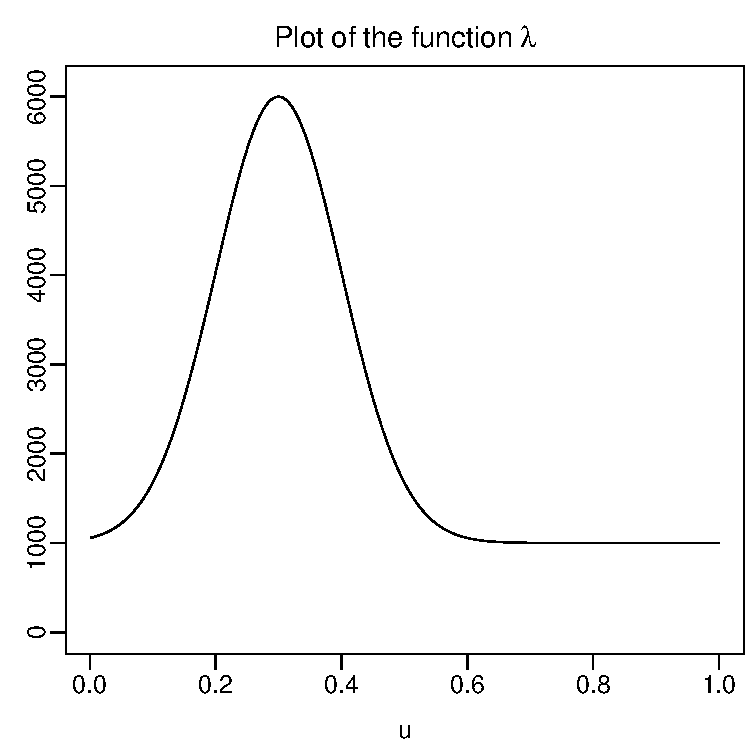
\includegraphics[width=\textwidth]{plots/lambda_fct}
\caption{}
\end{subfigure}\hspace{0.25cm}
\begin{subfigure}[b]{0.475\textwidth}
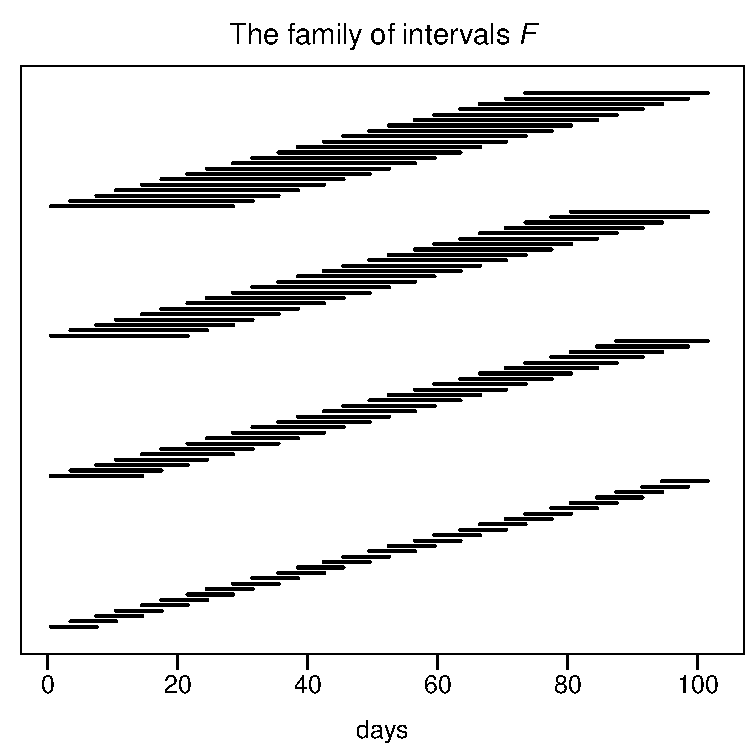
\includegraphics[width=\textwidth]{plots/all_intervals}
\caption{}
\end{subfigure}
\caption{(a) Plot of the function $\lambda$; (b) plot of the family $\intervals$.}\label{fig:lambda_F}
\end{figure}



%\noindent Simulation setting: 
%\begin{itemize}[label=--,leftmargin=0.5cm]

%\item We simulate data $\{X_{it}: 1 \le t \le T, \, 1 \le i \le n\}$ for different $n$ and $T$ from the model 
%\[ \X_{it} = \lambda_i\Big(\frac{t}{T}\Big) + \varepsilon_{it} \quad \text{with} \quad \varepsilon_{it} = \sigma \sqrt{\lambda_i\Big(\frac{t}{T}\Big)} \eta_{it}, \]
%where $\eta_{it}$ are i.i.d.\ standard normal. 

%\item We assume that $H_0^{(ijk)}$ holds true for all $(i,j,k)$ under consideration, implying that $\lambda_i = \lambda$ for all $i$. We in particular let
%\[ \lambda(u) = 5000 \exp\Big(-\frac{(x-3)^2}{2}\Big) + 50. \]
%This function has a similar form as the estimated curves in the application. Moreover, $\lambda(0) \approx 100$, which fits our normalization that each time series starts at the first day with more than $100$ new cases. 

%\item We set $\sigma = 10$. (We may also take something like 15 or 20.) (Estimates of $\sigma$ in the application take similar values.)

%\item We let $\pairs = \{ (i,j): 1 \le i < j \le n\}$ and $\intervals$ a family of intervals with $h_k \in \{ 7/T,14/T,21/T,28/T \}$. Hence, all intervals in $\intervals$ have length either 7 days (1 week), 14 days (2 weeks), 21 days (3 weeks), or 28 days (4 weeks) [we may even include longer intervals with 5, 6, etc.\ weeks]. For each length $h_k$, we include all intervals that start at days $t = 1 + 7(j-1)$ and $t = 4 + 7(j-1)$ for $j=1,2,\ldots$. A graphical presentation of the family of intervals $\intervals$ is given in Figure ??. 

%\item We may let $T \in \{50,100\}$ and $n \in \{5,10,50,100\}$. 

%\end{itemize}


\subsection{Analysis of COVID-19 data}\label{subsec:app}

\begin{figure}[t!]
\begin{subfigure}[b]{0.475\textwidth}
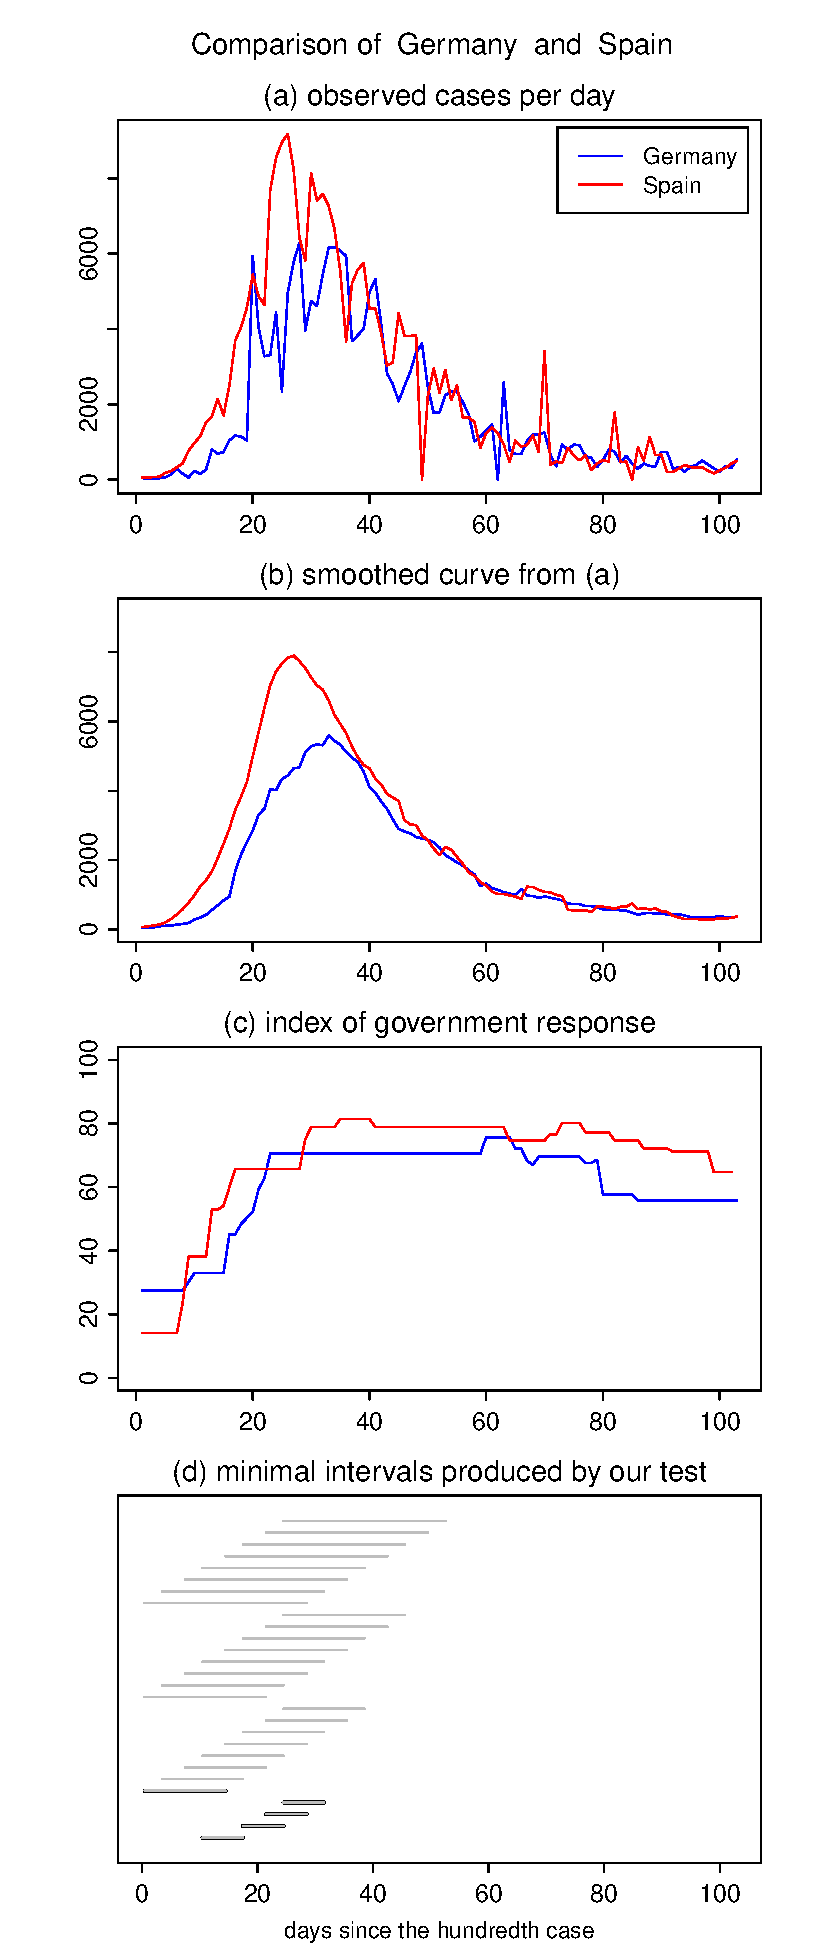
\includegraphics[width=\textwidth]{plots/DEU_vs_ESP}
\end{subfigure}\hspace{0.25cm}
\begin{subfigure}[b]{0.475\textwidth}
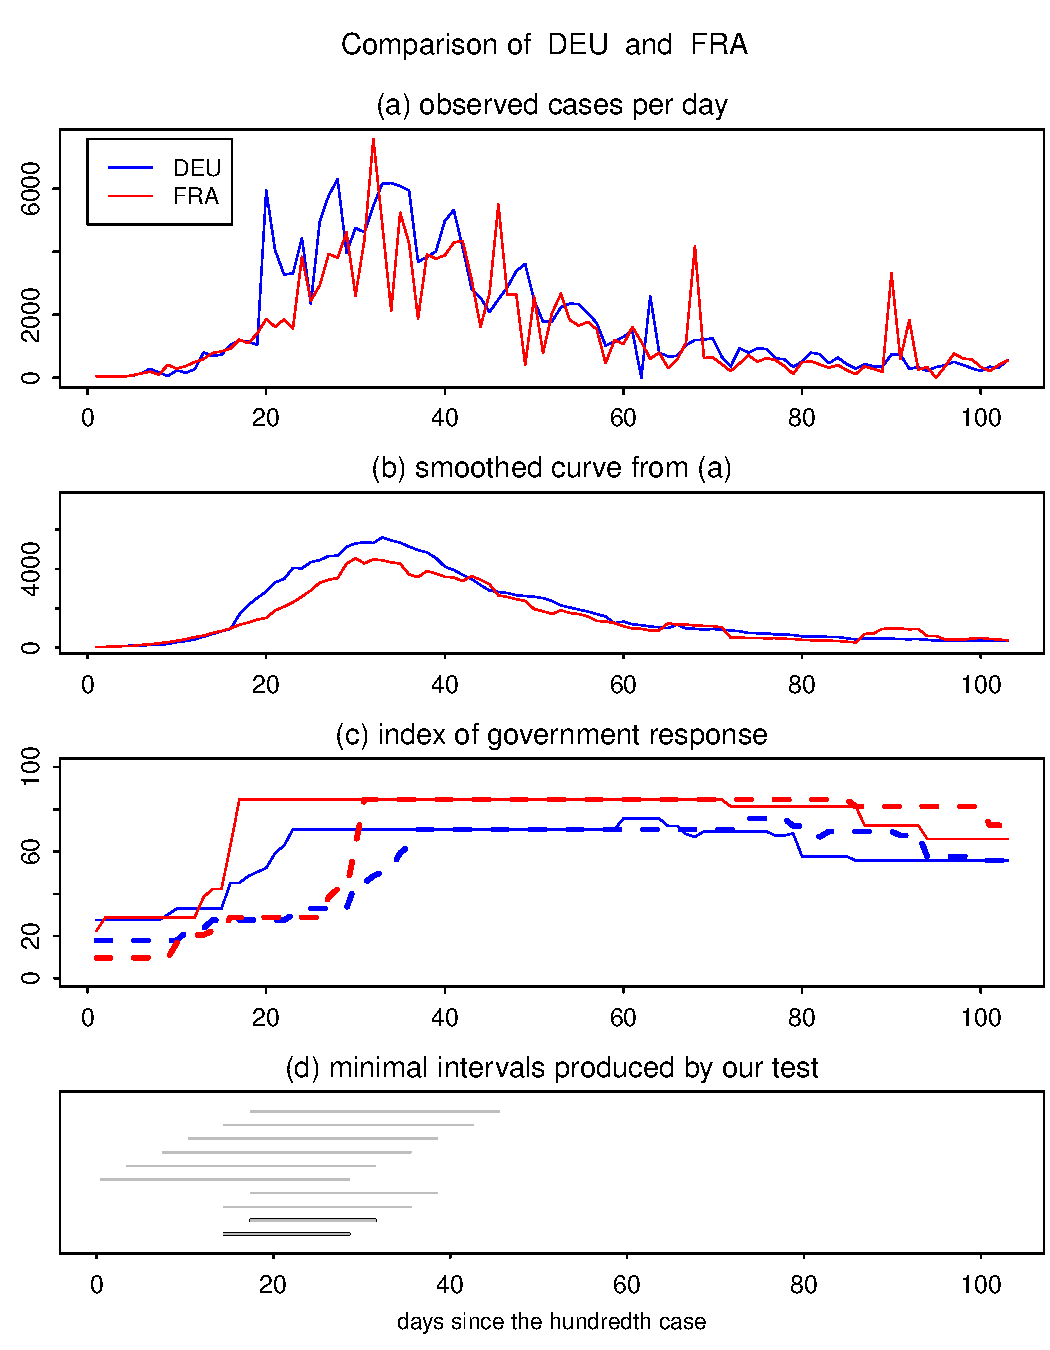
\includegraphics[width=\textwidth]{plots/DEU_vs_FRA}
\end{subfigure}
\vspace{0.25cm}
\begin{subfigure}[b]{0.475\textwidth}
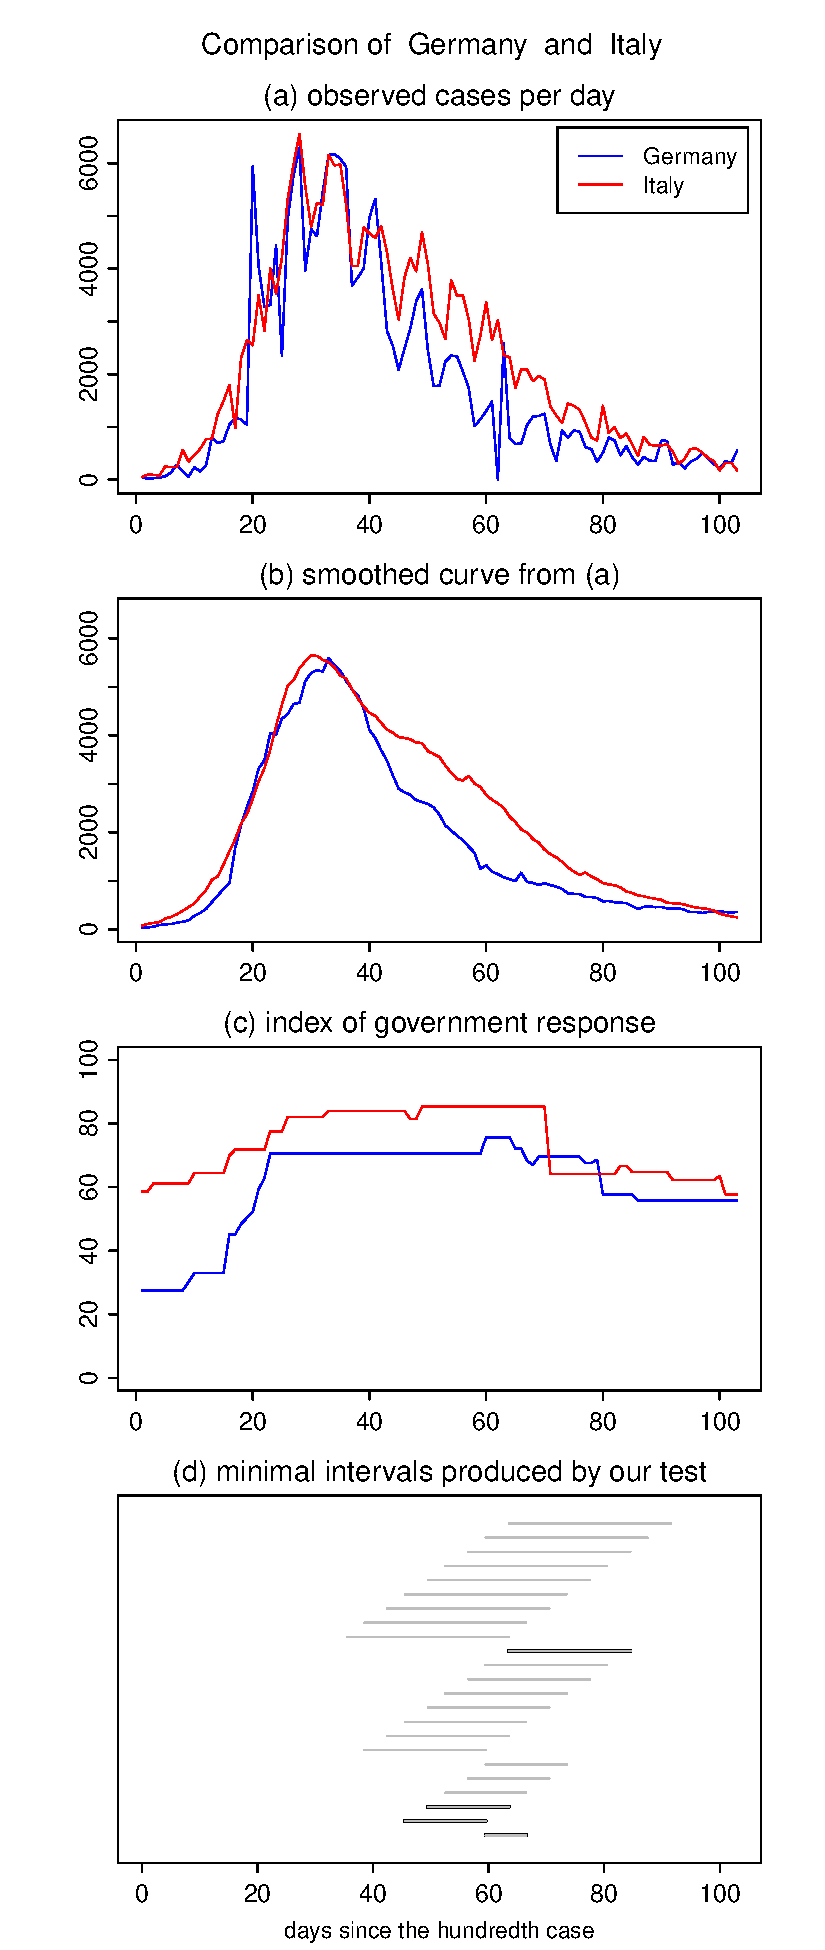
\includegraphics[width=\textwidth]{plots/DEU_vs_ITA}
\end{subfigure}\hspace{0.55cm}
\begin{subfigure}[b]{0.475\textwidth}
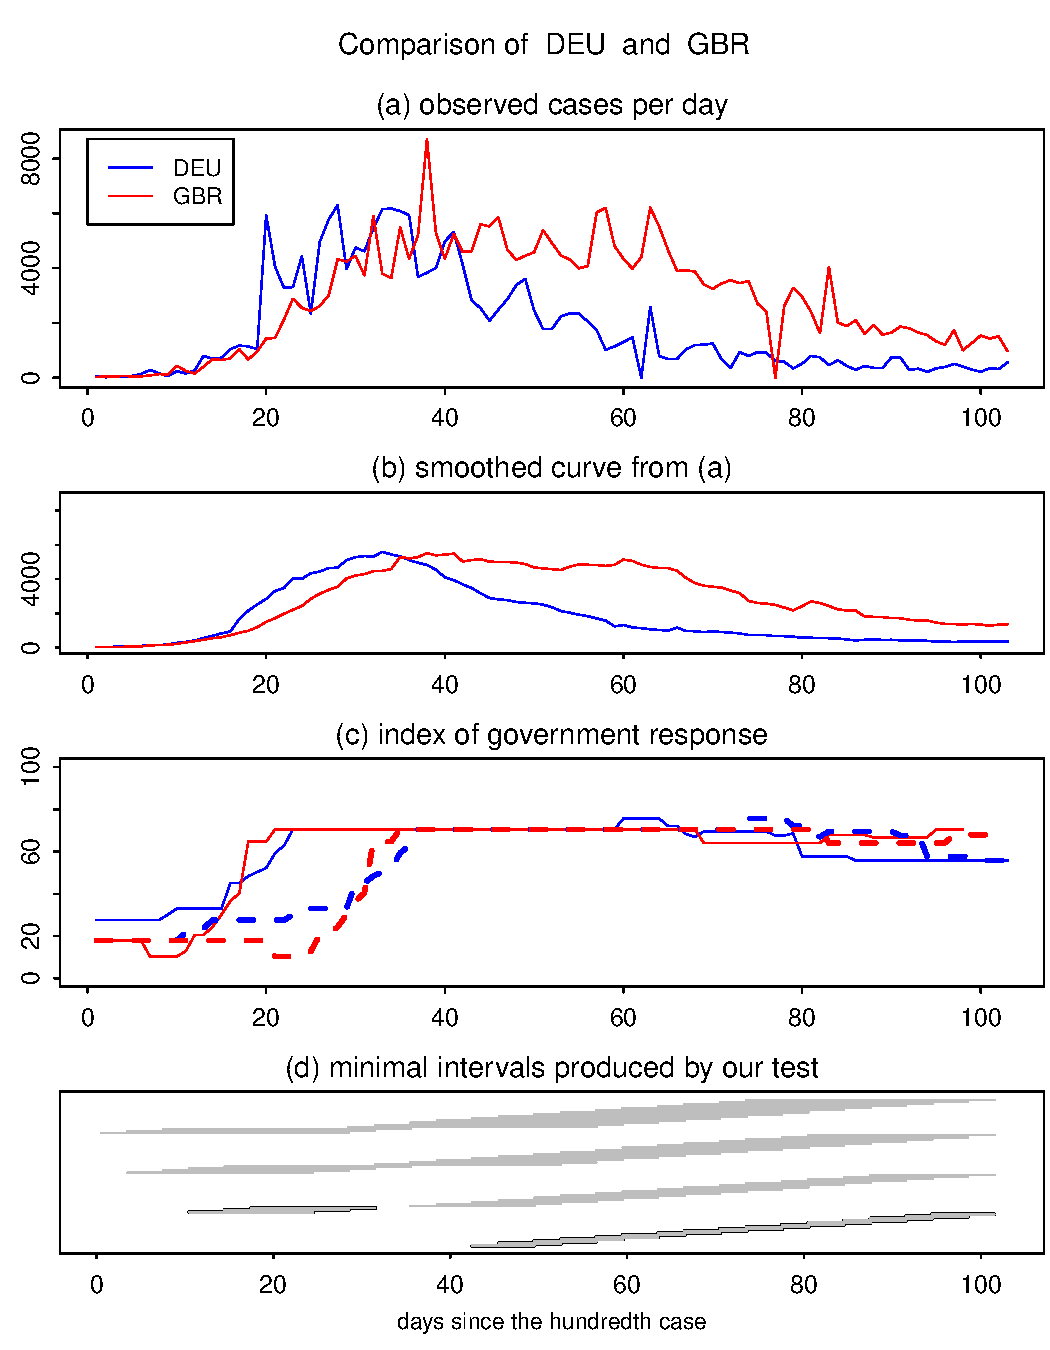
\includegraphics[width=\textwidth]{plots/DEU_vs_GBR}
\end{subfigure}
\end{figure}
\begin{figure}[t!]\ContinuedFloat
\begin{subfigure}[b]{0.475\textwidth}
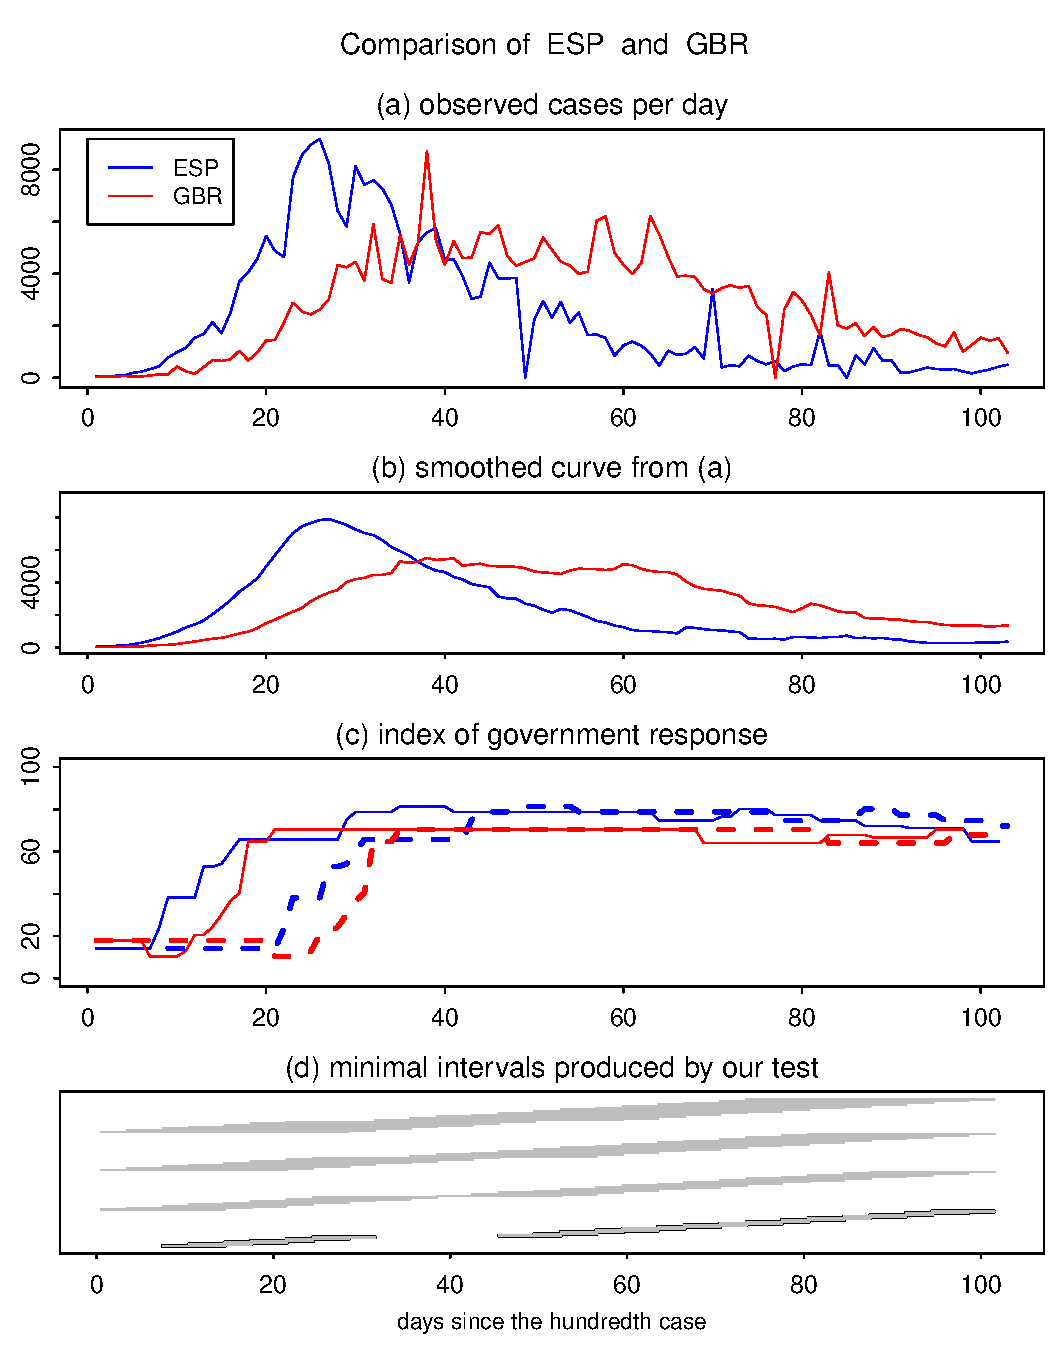
\includegraphics[width=\textwidth]{plots/ESP_vs_GBR}
\end{subfigure}\hspace{0.55cm}
\begin{subfigure}[b]{0.475\textwidth}
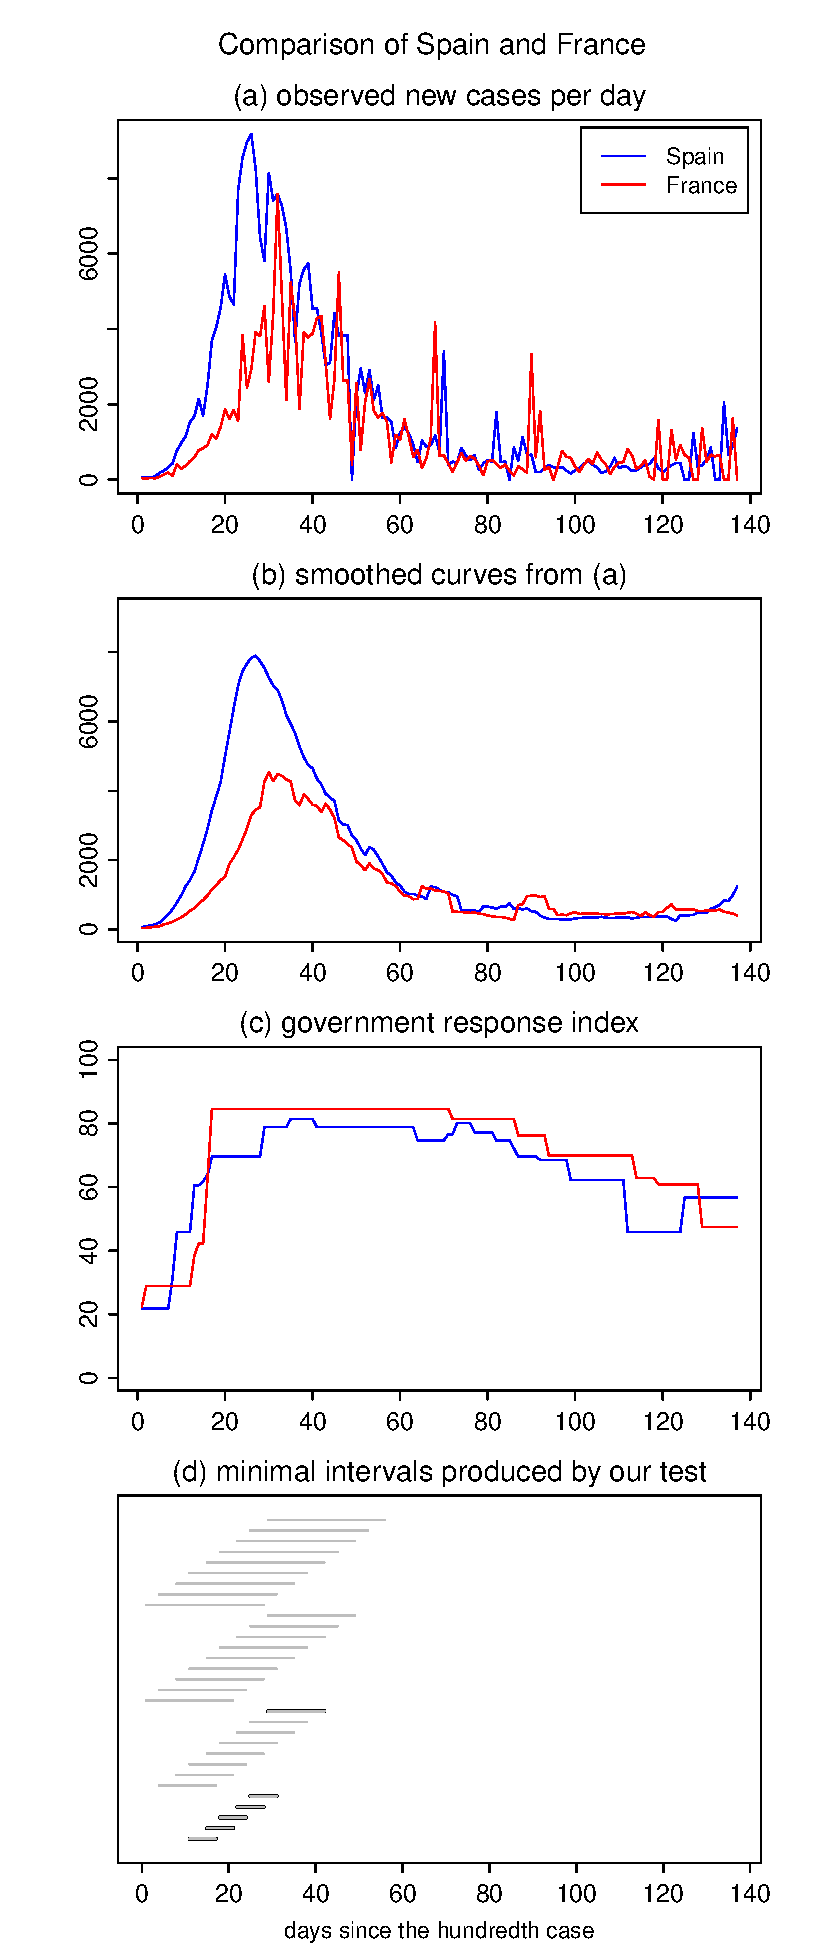
\includegraphics[width=\textwidth]{plots/ESP_vs_FRA}
\end{subfigure}
\vspace{0.25cm}
\begin{subfigure}[b]{0.475\textwidth}
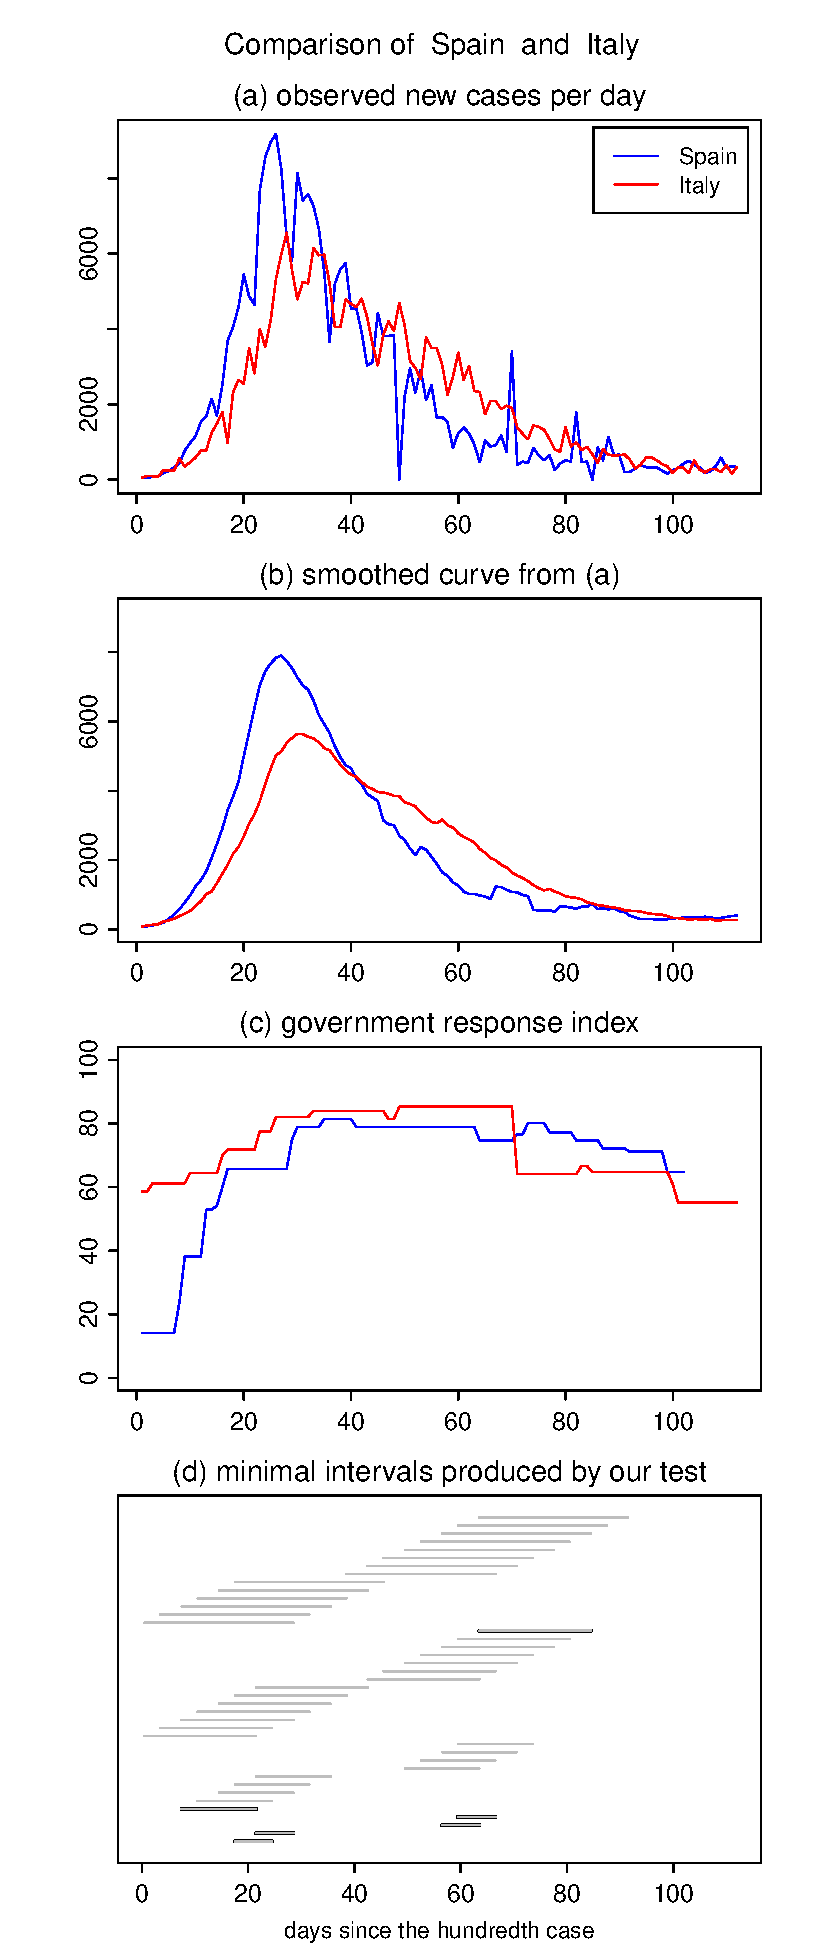
\includegraphics[width=\textwidth]{plots/ESP_vs_ITA}
\end{subfigure}\hspace{0.55cm}
\begin{subfigure}[b]{0.475\textwidth}
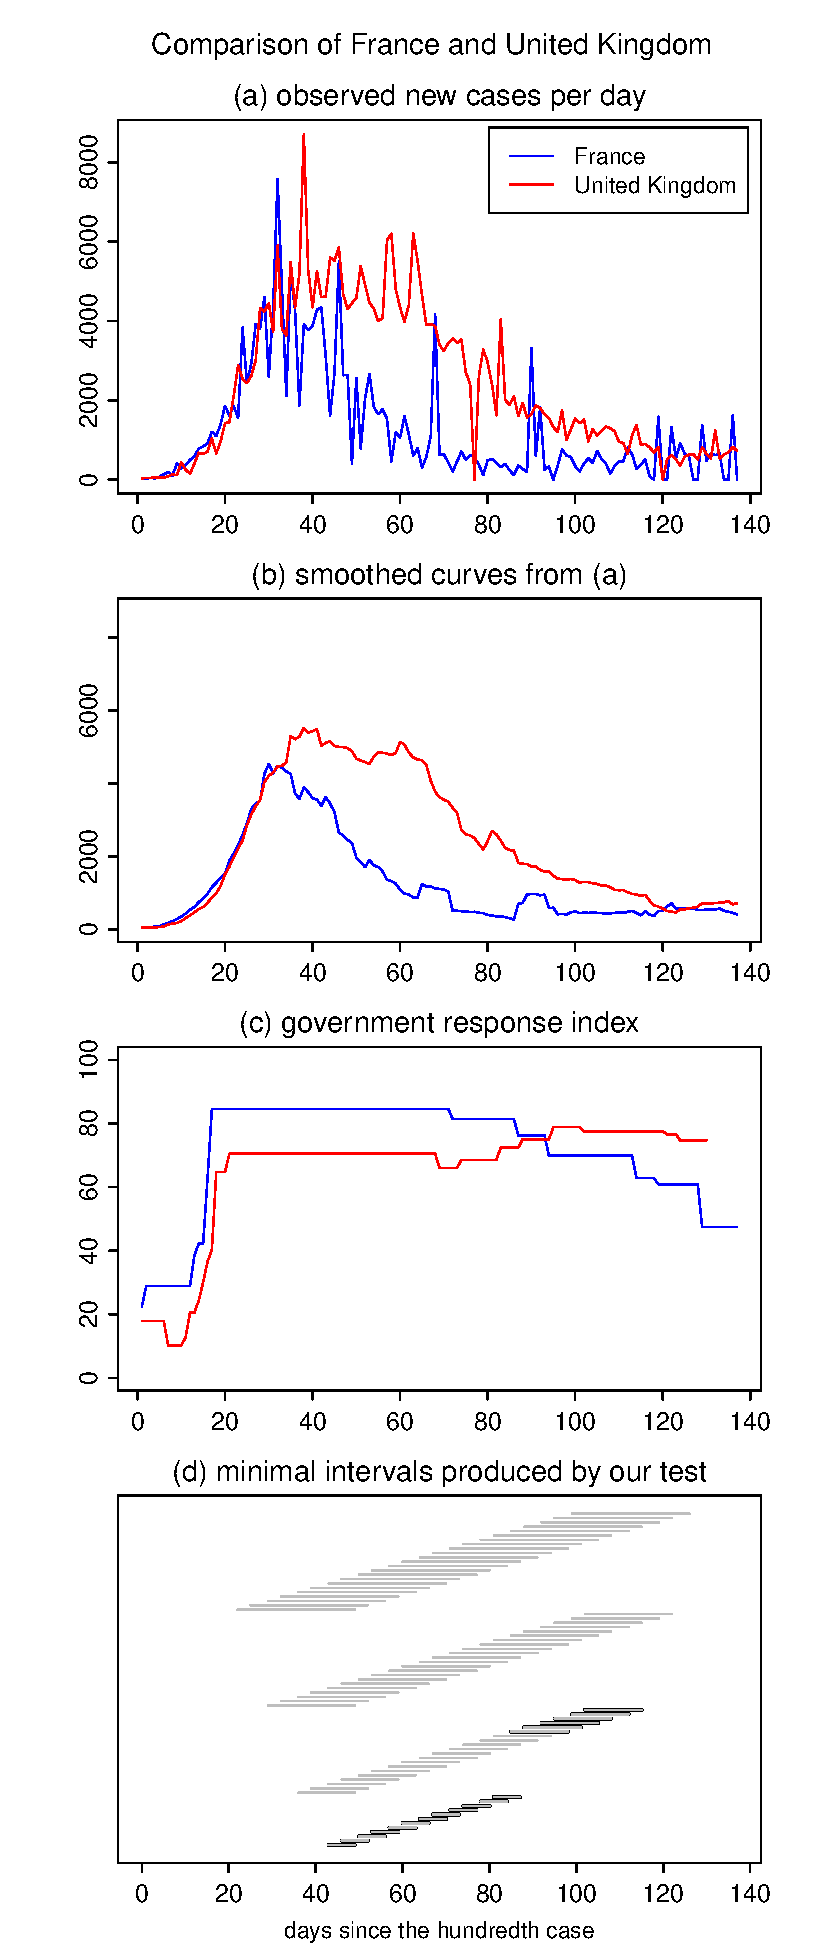
\includegraphics[width=\textwidth]{plots/FRA_vs_GBR}
\end{subfigure}
\end{figure}
\begin{figure}[t!]\ContinuedFloat
\begin{subfigure}[b]{0.475\textwidth}
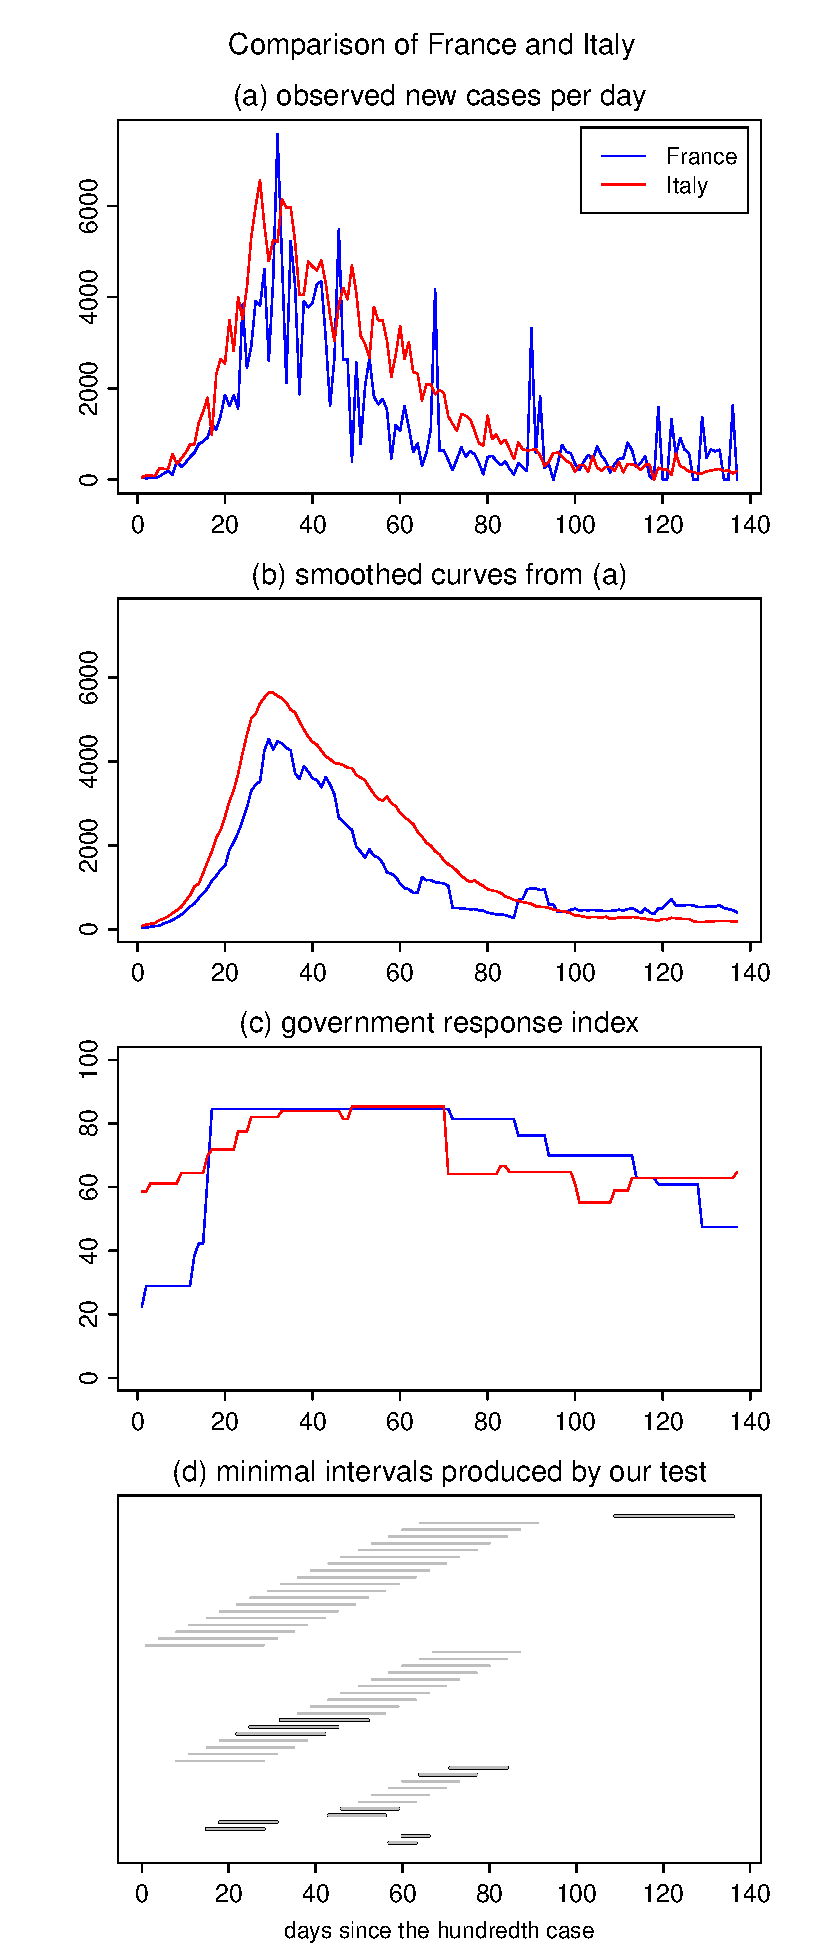
\includegraphics[width=\textwidth]{plots/FRA_vs_ITA}
\end{subfigure}\hspace{0.55cm}
\begin{subfigure}[b]{0.475\textwidth}
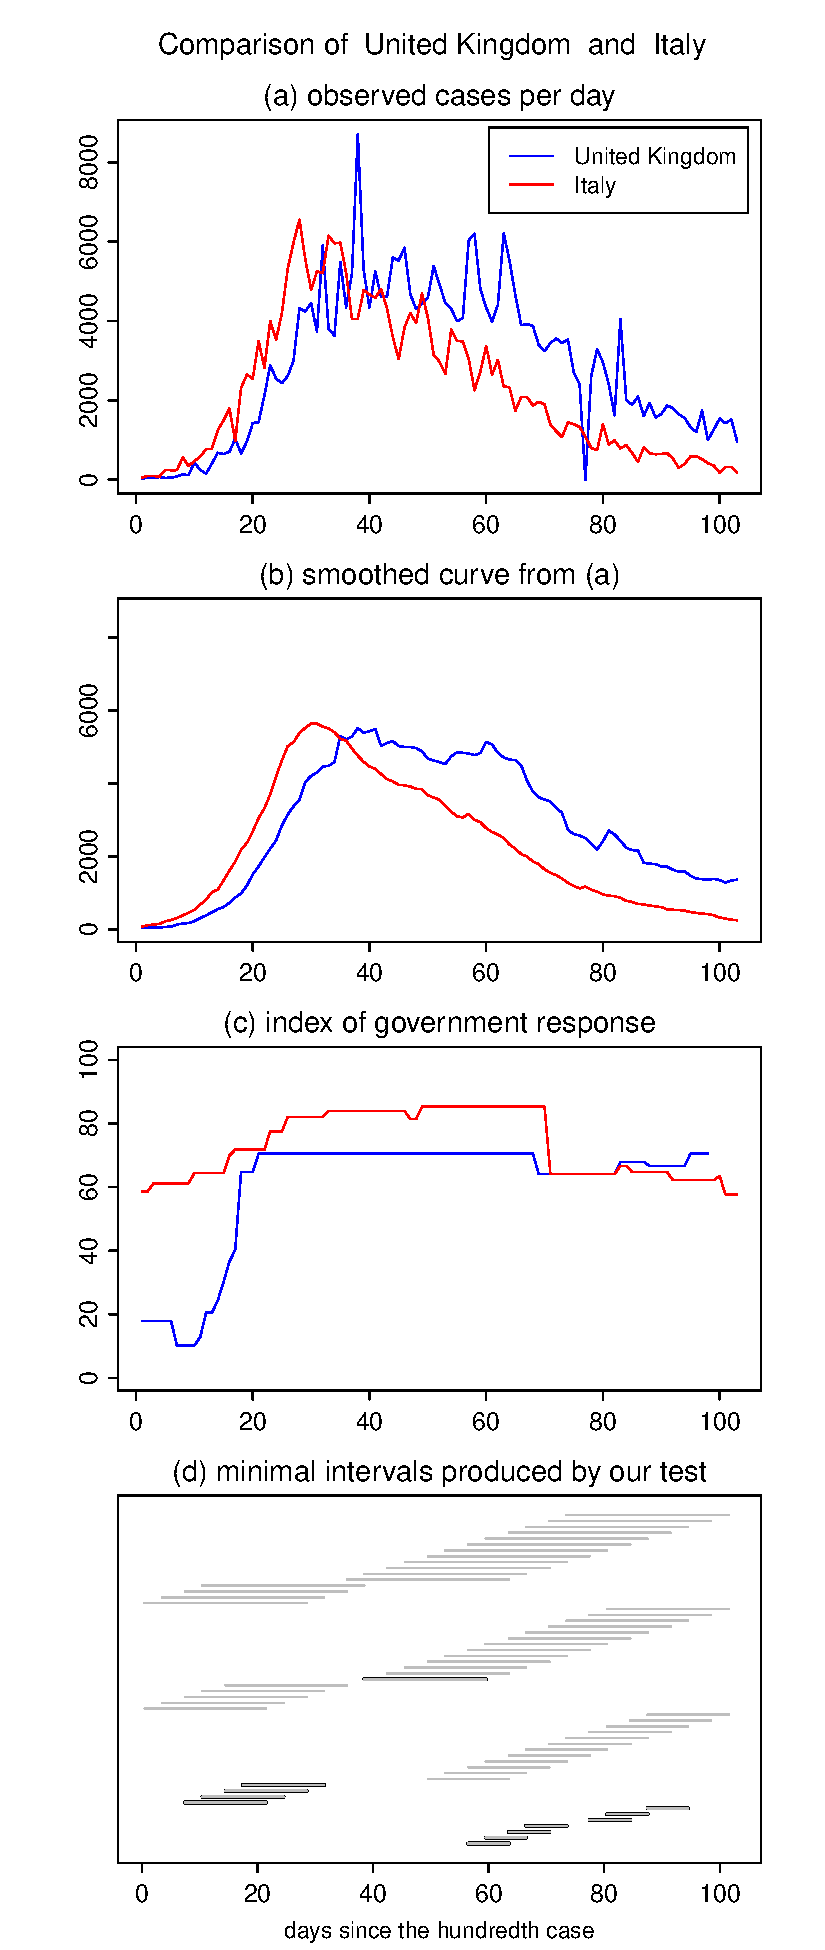
\includegraphics[width=\textwidth]{plots/GBR_vs_ITA}
\end{subfigure}
\vspace{0.25cm}

\caption{Summary of the results for the daily numbers of the new cases of COVID-19 in Germany, Spain, France, Italy and The United Kingdom with one subfigure corresponding to the results of one pairwise comparison of these countries. Panel (a) of each subfigure shows the two observed time series. Panel (b) in each subfigure shows the smoothed versions of the time series from (a) using the bandwidth of $7$ days. Panel (c) of each subfigure show the corresponding time series of the Government Response Index (solid line) against the lagged version of itself (dashed line), with lag being 14 days. Panel (d) of each subfigure depicts the set of intervals $\intervals_{\text{reject}}(i,j)$ in gray and the set of minimal intervals constructed on the basis of $\intervals_{\text{reject}}(i,j)$ in black.}\label{fig:MSE_slope10}
\end{figure}



\FloatBarrier



\newpage
\section*{A \hspace{0.2cm} Appendix}
\def\theequation{A.\arabic{equation}}
\setcounter{equation}{0}

\enlargethispage{0.1cm}


In what follows, we state and prove the main theoretical results on the multiscale test developed in Section \ref{sec:test}. Throughout the Appendix, we let $C$ be a generic positive constant that may take a different value on each occurrence. Unless stated differently, $C$ depends neither on the time series length $T$ nor on the dimension $p$ of the test problem. We further use the symbols $h_{\min}:= \min_{1 \le k \le K} h_k$ and $h_{\max} := \max_{1 \le k \le K} h_k$ to denote the smallest and largest interval length in the family $\intervals$. 


\begin{theoremA}\label{theo1}
Let \ref{C1} and \ref{C2} be satisfied. Moreover, assume that (i) $h_{\max} = o(1/\log T)$, (ii) $h_{\min} \ge CT^{-b}$ for some $b \in (0,1)$, and (iii) $p = O(T^{(\theta/2)(1-b)-(1+\delta)})$ for some small $\delta > 0$. Then for any given $\alpha \in (0,1)$,
\[ \textnormal{FWER}(\alpha) := \pr \Big( \exists (i,j,k) \in \indexset_0: |\hat{\psi}_{ijk,T}| > c_{T,\textnormal{Gauss}}(\alpha,h_k) \Big) \le \alpha + o(1), \]
where $\indexset_0 \subseteq \indexset$ is the set of all $(i,j,k) \in \indexset$ for which $H_0^{(ijk)}$ holds true. 
%Hence, the simultaneous test defined in \eqref{eq:test} asymptotically controls the FWER at level $\alpha$ for any given significance level $\alpha \in (0,1)$.
\end{theoremA}


\noindent According to Theorem \ref{theo1}, the multiscale test asymptotically controls the FWER at level $\alpha$ under conditions \ref{C1}--\ref{C2} and the restrictions (i)--(iii) on $h_{\min}$, $h_{\max}$ and $p$. %We briefly comment on the latter restrictions. 
Restriction (i) allows the maximal interval length $h_{\max}$ to converge to zero very slowly, which means that $h_{\max}$ can be picked very large in practice. According to restriction (ii), the minimal interval length $h_{\min}$ can be chosen to go to zero as any polynomial $T^{-b}$ with some $b \in (0,1)$. Restriction (iii) allows the dimension $p$ of the test problem to grow polynomially in $T$. Specifically, $p$ may grow at most as the polynomial $T^{\gamma}$ with $\gamma = (\theta/2)(1-b)-(1+\delta)$. As one can see, the exponent $\gamma$ depends on the number of error moments $\theta$ defined in \ref{C2} and the parameter $b$ that specifies the minimal interval length $h_{\min}$. In particular, for any given $b \in (0,1)$, the exponent $\gamma$ gets larger as $\theta$ increases. Hence, the larger the number of error moments $\theta$, the faster $p$ may grow in comparison to $T$. In the extreme case where all error moments exist, that is, where $\theta$ can be made as large as desired, $p$ may grow as any polynomial of $T$, no matter how we pick $b \in (0,1)$. Thus, if the error terms have sufficiently many moments, the dimension $p$ can be extremely large in comparison to $T$ and the minimal interval length $h_{\min}$ can be chosen very small. 
%Restriction (i) allows the maximal interval length $h_{\max}$ to converge to zero very slowly, which means that $h_{\max}$ can be picked very large in practice. According to restrictions (ii) and (iii), the minimal interval length $h_{\min}$ is intertwined with the dimension $p$ of the test problem, which in turn depends on the number of error moments $\theta$ specified in \ref{C2}. As an example, if $\theta > 8$ and $h_{\min} = CT^{-b}$ with $b=1/4$, then we require that $p \le T^2$. More generally speaking, the larger the number of moments $\theta$, the larger $p$ can be compared to $T$ for a given exponent $b$. In the extreme case where all error moments exist, that is, where $\theta$ can be made as large as desired, $p$ may grow as any polynomial of $T$ with arbitrarily large exponent and $b$ can be chosen as any fixed constant in the interval $(0,1)$. Hence, if the error terms have sufficiently many moments, the overall dimension $p$ of the test problem can be extremely large compared to $T$ and the minimal interval length $h_{\min}$ can be extremely small. 


The following corollary is an immediate consequence of Theorem \ref{theo1}. It provides the theoretical justification needed to make simultaneous confidence statements of the form \eqref{eq:confidencestatement1}--\eqref{eq:confidencestatement3}.


\begin{corollaryA}\label{corollary1}
Under the conditions of Theorem \ref{theo1}, 
\[ \pr\Big( \forall (i,j,k) \in \indexset: \text{ If } |\hat{\psi}_{ijk,T}| > c_{T,\textnormal{Gauss}}(\alpha,h_k), \text{ then } (i,j,k) \notin \indexset_0 \Big) \ge 1 - \alpha + o(1) \]
for any given $\alpha \in (0,1)$.   
%Hence, with asymptotic probability at least $1-\alpha$, the two intensity functions $\lambda_i$ and $\lambda_j$ differ on the interval $\mathcal{I}_k$ for all $(i,j,k) \in \indexset$ for which the test rejects $H_0^{(ijk)}$. 
\end{corollaryA} 


\begin{proof}[\textnormal{\textbf{Proof of Theorem \ref{theo1}.}}] The proof proceeds in several steps. 
\begin{enumerate}[label=\textit{Step \arabic*.}, leftmargin=0cm, itemindent=1.45cm]


\item Let $\hat{\Psi}_T = \max_{(i,j,k) \in \indexset} a_k (|\hat{\psi}_{ijk,T}^0| - b_k)$ with $\hat{\psi}_{ijk,T}^0$ introduced in \eqref{eq:stat0} and define $\Psi_T = \max_{(i,j,k) \in \indexset} a_k (|\psi_{ijk,T}^0| - b_k)$ with 
\[ \psi_{ijk,T}^0 = \frac{1}{\sqrt{2Th_k}} \sum\limits_{t=1}^T \ind\Big(\frac{t}{T} \in \mathcal{I}_k\Big) (\eta_{it} - \eta_{jt}). \]
To start with, we prove that  
\begin{equation}\label{eq:approxerror1}
\big| \hat{\Psi}_T - \Psi_T \big| = o_p(r_T),
\end{equation}
where $\{r_T\}$ is any null sequence that converges more slowly to zero than $\rho_T = \sqrt{\log T} \{ \log p/\sqrt{Th_{\min}} + h_{\max} \sqrt{\log p} \}$, that is, $\rho_T/r_T \rightarrow 0$ as $T \rightarrow \infty$. Since the proof of \eqref{eq:approxerror1} is rather technical and lengthy, the details are provided in the Supplementary Material. 


\item We next prove that 
\begin{equation}\label{eq:kolmogorov-distance}
\sup_{q \in \reals} \Big| \pr \big( \Psi_T \le q \big) - \pr \big( \Phi_T \le q \big) \Big| = o(1).
\end{equation}
To do so, we rewrite the statistics $\Psi_T$ and $\Phi_T$ as follows: Define 
\begin{equation*}
V^{(ijk)}_t = V^{(ijk)}_{t,T} := \sqrt{\frac{T}{2Th_k}} \ind\Big(\frac{t}{T} \in \mathcal{I}_k\Big) (\eta_{it} - \eta_{jt})
\end{equation*}
for $(i,j,k) \in \indexset$ and let $\boldsymbol{V}_t = (V_t^{(ijk)}: (i,j,k) \in \indexset)$ be the $p$-dimensional random vector with the entries $V_t^{(ijk)}$. With this notation, we get that $\psi_{ijk,T}^0 = T^{-1/2} \sum_{t=1}^T V^{(ijk)}_t$ and thus 
\begin{align*}
\Psi_T 
 & = \max_{(i,j,k) \in \indexset}  a_k \big( |\psi_{ijk,T}^0| - b_k \big) \\
 & = \max_{(i,j,k) \in \indexset} a_k \Big\{ \Big|\frac{1}{\sqrt{T}} \sum_{t=1}^T V^{(ijk)}_t\Big| - b_k \Big\}.
\end{align*} 
Analogously, we define 
\begin{equation*}
W^{(ijk)}_t = W^{(ijk)}_{t,T} := \sqrt{\frac{T}{2Th_k}} \ind\Big(\frac{t}{T} \in \mathcal{I}_k\Big) (Z_{it} - Z_{jt})
\end{equation*}
with $Z_{it}$ i.i.d.\ standard normal and let $\boldsymbol{W}_t = (W_t^{(ijk)}: (i,j,k) \in \indexset)$. The vector $\boldsymbol{W}_t$ is a Gaussian version of $\boldsymbol{V}_t$ with the same mean and variance. In particular, $\ex[\boldsymbol{W}_t] = \ex[\boldsymbol{V}_t] = 0$ and $\ex[\boldsymbol{W}_t \boldsymbol{W}_t^\top] = \ex[\boldsymbol{V}_t \boldsymbol{V}_t^\top]$. Similarly as before, we can write $\phi_{ijk,T} = T^{-1/2} \sum_{t=1}^T W^{(ijk)}_t$ and  
\begin{align*}
\Phi_T 
 & = \max_{(i,j,k) \in \indexset} a_k \big( |\phi_{ijk,T}| - b_k \big) \\
 & = \max_{(i,j,k) \in \indexset} a_k \Big\{ \Big|\frac{1}{\sqrt{T}} \sum_{t=1}^T W^{(ijk)}_t\Big| - b_k \Big\}.
\end{align*} 
For any $q \in \reals$, it holds that
\begin{align*}
\pr \big( \Psi_T \le q \big) 
 & = \pr \Big( \max_{(i,j,k) \in \indexset} a_k \Big\{ \Big|\frac{1}{\sqrt{T}} \sum_{t=1}^T V^{(ijk)}_t\Big| - b_k \Big\} \le q \Big) \\
 & = \pr \Big( \Big|\frac{1}{\sqrt{T}} \sum_{t=1}^T V^{(ijk)}_t\Big| \le q_{ijk} \text{ for all } (i,j,k) \in \indexset \Big) \\
 & = \pr \Big( \Big|\frac{1}{\sqrt{T}} \sum_{t=1}^T \boldsymbol{V}_t\Big| \le \boldsymbol{q} \Big),
\end{align*} 
where $\boldsymbol{q}$ is the $\reals^p$-vector with the entries $q_{ijk} = q/a_k + b_k$. Analogously, we have  
\[ \pr \big( \Phi_T \le q \big) = \pr \Big( \Big|\frac{1}{\sqrt{T}} \sum_{t=1}^T \boldsymbol{W}_t\Big| \le \boldsymbol{q} \Big). \]
With this notation at hand, we can make use of Proposition 2.1 from \cite{Chernozhukov2017}. In our context, this proposition can be stated as follows: 
\begin{propA}\label{prop:Chernozhukov}
Assume that 
\begin{enumerate}[label=(\alph*),leftmargin=0.7cm]
\item $T^{-1} \sum_{t=1}^T \ex (V^{(ijk)}_t)^2 \ge \delta > 0$ for all $(i,j,k) \in \indexset$.
\item $T^{-1} \sum_{t=1}^T \ex[ |V^{(ijk)}_t|^{2+r} ] \le B_T^r$ for all $(i,j,k) \in \indexset$ and $r=1,2$, where $B_T \ge 1$ are constants that may tend to infinity as $T \rightarrow \infty$.  
\item $\ex[ \{ \max_{(i,j,k) \in \indexset} |V^{(ijk)}_t| / B_T \}^\theta ] \le 2$ for all $t$ and some $\theta > 4$.  
\end{enumerate}
Then  
\begin{align}
\sup_{\boldsymbol{q} \in \reals^p} \Big| \pr \Big( \Big|\frac{1}{\sqrt{T}} \sum_{t=1}^T \boldsymbol{V}_t\Big| \le \boldsymbol{q} \Big) & - \pr \Big( \Big|\frac{1}{\sqrt{T}} \sum_{t=1}^T \boldsymbol{W}_t\Big| \le \boldsymbol{q} \Big) \Big| \nonumber \\ & \le C \Big\{ \Big( \frac{B_T^2 \log^7(pT)}{T} \Big)^{1/6} + \Big( \frac{B_T^2 \log^3(pT)}{T^{1-2/\theta}} \Big)^{1/3} \Big\}, \label{eq:Chernozhukov}
\end{align}
where $C$ depends only on $\delta$ and $\theta$. 
\end{propA}
It is straightforward to verify that assumptions (a)--(c) are satisfied under the conditions of Theorem \ref{theo1} for sufficiently large $T$, where $B_T$ can be chosen as $B_T = C p^{1/\theta} h_{\min}^{-1/2}$ with $C$ sufficiently large. Moreover, it can be shown that the right-hand side of \eqref{eq:Chernozhukov} is $o(1)$ for this choice of $B_T$. Hence, Proposition \ref{prop:Chernozhukov} yields that 
\[ \sup_{\boldsymbol{q} \in \reals^p} \Big| \pr \Big( \Big|\frac{1}{\sqrt{T}} \sum_{t=1}^T \boldsymbol{V}_t\Big| \le \boldsymbol{q} \Big) - \pr \Big( \Big|\frac{1}{\sqrt{T}} \sum_{t=1}^T \boldsymbol{W}_t\Big| \le \boldsymbol{q} \Big) \Big| = o(1), \]
which in turn implies \eqref{eq:kolmogorov-distance}. 


\item With the help of \eqref{eq:approxerror1} and \eqref{eq:kolmogorov-distance}, we now show that 
\begin{equation}\label{eq:kolmogorov-distance-hat}
\sup_{q \in \reals} \Big| \pr \big( \hat{\Psi}_T \le q \big) - \pr \big( \Phi_T \le q \big) \Big| = o(1).
\end{equation}
To start with, the above supremum can be bounded by 
\begin{align*}
 & \sup_{q \in \reals} \Big| \pr \big( \hat{\Psi}_T \le q \big) - \pr \big( \Phi_T \le q \big) \Big| \\
 & = \sup_{q \in \reals} \Big| \pr \Big( \Psi_T \le q + \big\{ \Psi_T - \hat{\Psi}_T \big\} \Big) - \pr \big( \Phi_T \le q \big) \Big| \\
 & \le \max \Big\{ \sup_{q \in \reals} \Big| \pr \Big( \Psi_T \le q + \big| \Psi_T - \hat{\Psi}_T \big| \Big) - \pr \big( \Phi_T \le q \big) \Big|, \\
 & \phantom{ \le \max \Big\{ \, } \sup_{q \in \reals} \Big| \pr \Big( \Psi_T \le q - \big| \Psi_T - \hat{\Psi}_T \big| \Big) - \pr \big( \Phi_T \le q \big) \Big| \Big\} \\
 & \le \max \Big\{ \sup_{q \in \reals} \Big| \pr \Big( \Psi_T \le q + r_T \Big) - \pr \big( \Phi_T \le q \big) \Big| +  \pr \Big( \big| \Psi_T - \hat{\Psi}_T \big| > r_T \Big), \\*
 & \phantom{ \le \max \Big\{ \, } \sup_{q \in \reals} \Big| \pr \Big( \Psi_T \le q - r_T \Big) - \pr \big( \Phi_T \le q \big) \Big| +  \pr \Big( \big| \Psi_T - \hat{\Psi}_T \big| > r_T \Big) \Big\}. 
\end{align*}
Moreover, 
\begin{align*}
 & \sup_{q \in \reals} \Big| \pr \Big( \Psi_T \le q \pm r_T \Big) - \pr \big( \Phi_T \le q \big) \Big| +  \pr \Big( \big| \Psi_T - \hat{\Psi}_T \big| > r_T \Big) \\
 & \le \sup_{q \in \reals} \Big| \pr \Big( \Psi_T \le q \pm r_T \Big) - \pr \Big( \Phi_T \le q \pm r_T \Big) \Big| \\
 & \quad + \sup_{q \in \reals} \Big| \pr \Big( \Phi_T \le q \pm r_T \Big) - \pr \big( \Phi_T \le q \big) \Big| + \pr \Big( \big| \Psi_T - \hat{\Psi}_T \big| > r_T \Big) \\
 & = \sup_{q \in \reals} \Big| \pr \Big( \Phi_T \le q \pm r_T \Big) - \pr \big( \Phi_T \le q \big) \Big| + o(1), 
\end{align*}
where the last line follows from \eqref{eq:approxerror1} and \eqref{eq:kolmogorov-distance}. Finally, by Nazarov's inequality (cp.\ \citeauthor{Nazarov2003}, \citeyear{Nazarov2003} and Lemma A.1 in \citeauthor{Chernozhukov2017}, \citeyear{Chernozhukov2017}),   
\begin{align*} 
 & \sup_{q \in \reals} \Big| \pr \Big( \Phi_T \le q \pm r_T \Big) - \pr \big( \Phi_T \le q \big) \Big| \\*
 & = \sup_{\boldsymbol{q} \in \reals^p} \Big| \pr \Big( \Big|\frac{1}{\sqrt{T}} \sum_{t=1}^T \boldsymbol{W}_t\Big| \le \boldsymbol{q} \pm r_T \Big) - \pr \Big( \Big|\frac{1}{\sqrt{T}} \sum_{t=1}^T \boldsymbol{W}_t\Big| \le \boldsymbol{q} \Big) \Big| \le C r_T \sqrt{\log(2 p)}, 
\end{align*}
where $C$ is a constant that depends only on the parameter $\delta$ defined in condition (a) of Proposition \ref{prop:Chernozhukov}.


\item By definition of the quantile $q_{T,\text{Gauss}}(\alpha)$, it holds that $\pr(\Phi_T \le q_{T,\text{Gauss}}(\alpha)) \ge 1-\alpha$. As shown in the Supplementary Material, we even have that  
\begin{equation}\label{eq:quant-exact}
\pr(\Phi_T \le q_{T,\text{Gauss}}(\alpha)) = 1-\alpha
\end {equation} 
for any $\alpha \in (0,1)$. From this and \eqref{eq:kolmogorov-distance-hat}, it immediately follows that  
\begin{equation}\label{eq:probbound-Psihat}
\pr \big( \hat{\Psi}_T \le q_{T,\text{Gauss}}(\alpha) \big) = 1 - \alpha + o(1), 
\end{equation}
which in turn yields the statement of Theorem \ref{theo1}. \qedhere


\end{enumerate}
\end{proof}


\begin{proof}[\textnormal{\textbf{Proof of Corollary \ref{corollary1}.}}]
By Theorem \ref{theo1}, 
\begin{align*}
1 - \alpha + o(1) 
 & \le 1 - \textnormal{FWER}(\alpha) \\
 & = \pr \Big( \nexists (i,j,k) \in \indexset_0: |\hat{\psi}_{ijk,T}| > c_{T,\textnormal{Gauss}}(\alpha,h_k) \Big) \\
 & = \pr\Big( \forall (i,j,k) \in \indexset: \text{ If } |\hat{\psi}_{ijk,T}| > c_{T,\textnormal{Gauss}}(\alpha,h_k), \text{ then } (i,j,k) \notin \indexset_0 \Big),
\end{align*}
which gives the statement of Corollary \ref{corollary1}.
\end{proof}



\bibliographystyle{ims}
{\small
\setlength{\bibsep}{0.45em}
\bibliography{bibliography}}



\newpage
\section*{S \hspace{0.2cm} Supplementary Material}
\def\theequation{S.\arabic{equation}}
\setcounter{equation}{0}


In what follows, we provide the technical details omitted in the Appendix. To start with, we prove the following auxiliary lemma.
\begin{lemmaS}\label{lemmaS1}
Under the conditions of Theorem \ref{theo1}, it holds that 
\[ \big| \hat{\sigma}^2 - \sigma^2 \big| = O_p\Big( \sqrt{\frac{\log p}{T}} \Big). \]
\end{lemmaS} 


\begin{proof}[\textnormal{\textbf{Proof of Lemma \ref{lemmaS1}.}}]
By definition, $\hat{\sigma}^2 = |\countries|^{-1} \sum_{i \in \countries} \hat{\sigma}_i^2$ and $\hat{\sigma}_i^2 = \{\sum_{t=2}^T (\X_{it}-\X_{it-1})^2\}\{2 \sum_{t=1}^T \X_{it}\}$. It holds that 
\begin{equation}\label{eq:approxerror:claim3:expansion}
\frac{1}{T} \sum\limits_{t=2}^T (X_{it} - X_{it-1})^2 = \frac{\sigma^2}{T} \sum\limits_{t=2}^T \lambda_i\Big(\frac{t}{T}\Big) (\eta_{it} - \eta_{it-1})^2 + \big\{R_{i,T}^{(1)} + \ldots + R_{i,T}^{(5)}\big\},
\end{equation}
where
\begin{align*}
R_{i,T}^{(1)} & = \frac{2\sigma}{T} \sum\limits_{t=2}^T \Big( \lambda_i\Big(\frac{t}{T}\Big) - \lambda_i\Big(\frac{t-1}{T}\Big) \Big) \sqrt{\lambda_i\Big(\frac{t}{T}\Big)} (\eta_{it} - \eta_{it-1}) \\
R_{i,T}^{(2)} & = \frac{2\sigma^2}{T} \sum\limits_{t=2}^T \Big( \sqrt{\lambda_i\Big(\frac{t}{T}\Big)} - \sqrt{\lambda_i\Big(\frac{t-1}{T}\Big)} \Big) \sqrt{\lambda_i\Big(\frac{t}{T}\Big)} \eta_{it-1} (\eta_{it} - \eta_{it-1}) \\
R_{i,T}^{(3)} & = \frac{1}{T} \sum\limits_{t=2}^T \Big( \lambda_i\Big(\frac{t}{T}\Big) - \lambda_i\Big(\frac{t-1}{T}\Big) \Big)^2 \\
R_{i,T}^{(4)} & = \frac{2 \sigma}{T} \sum\limits_{t=2}^T \Big( \lambda_i\Big(\frac{t}{T}\Big) - \lambda_i\Big(\frac{t-1}{T}\Big) \Big) \Big( \sqrt{\lambda_i\Big(\frac{t}{T}\Big)} - \sqrt{\lambda_i\Big(\frac{t-1}{T}\Big)} \Big) \eta_{it-1} \\
R_{i,T}^{(5)} & = \frac{\sigma^2}{T} \sum\limits_{t=2}^T  \Big( \sqrt{\lambda_i\Big(\frac{t}{T}\Big)} - \sqrt{\lambda_i\Big(\frac{t-1}{T}\Big)} \Big)^2 \eta_{it-1}^2.
\end{align*} 
With the help of an exponential inequality and standard arguments, it can be shown that 
\[ \max_{i \in \countries} \Big| \frac{1}{T} \sum_{t=1}^T w_i\Big(\frac{t}{T}\Big) \big\{ g(\eta_{it}) - \ex g(\eta_{it}) \big\} \Big| = O_p\Big( \sqrt{\frac{\log p}{T}} \Big), \]
where we let $g(x) = x$, $g(x) = |x|$ or $g(x) = x^2$, and $w_i(t/T)$ are deterministic weights with the property that $|w_i(t/T)| \le w_{\max} < \infty$ for all $i$, $t$ and $T$ and some positive constant $w_{\max}$. Using this uniform convergence result along with conditions \ref{C1} and \ref{C2}, we obtain that 
\[ \max_{i \in \countries} \Big| \frac{1}{T} \sum\limits_{t=2}^T \lambda_i\Big(\frac{t}{T}\Big) (\eta_{it} - \eta_{it-1})^2 - \frac{2}{T} \sum\limits_{t=1}^T \lambda_i\Big(\frac{t}{T}\Big) \Big| = O_p\Big( \sqrt{\frac{\log p}{T}} \Big) \]
and 
\[ \max_{1 \le \ell \le 5} \max_{i \in \countries} |R_{i,T}^{(\ell)}| = O_p(T^{-1}). \]
Applying these two statements to \eqref{eq:approxerror:claim3:expansion}, we can infer that
\begin{equation}\label{eq:approxerror:claim2:1}
\max_{i \in \countries} \Big| \frac{1}{T} \sum\limits_{t=2}^T (X_{it} - X_{it-1})^2 - \frac{2}{T} \sum\limits_{t=1}^T \lambda_i\Big(\frac{t}{T}\Big) \Big| = O_p\Big( \sqrt{\frac{\log p}{T}} \Big). 
\end{equation}
By similar but simpler arguments, we additionally get that 
\begin{equation}\label{eq:approxerror:claim2:2}
\max_{i \in \countries} \Big| \frac{1}{T} \sum\limits_{t=1}^T X_{it} - \frac{1}{T} \sum\limits_{t=1}^T \lambda_i\Big(\frac{t}{T}\Big) \Big| = O_p\Big( \sqrt{\frac{\log p}{T}} \Big). 
\end{equation}
From \eqref{eq:approxerror:claim2:1} and \eqref{eq:approxerror:claim2:2}, it follows that $\max_{i \in \countries} |\hat{\sigma}_i^2 - \sigma^2| = O_p(\sqrt{\log p / T})$, which in turn implies that $|\hat{\sigma}^2 - \sigma^2| = O_p(\sqrt{\log p / T})$ as well. 
\end{proof} 


\begin{proof}[\textnormal{\textbf{Proof of (\ref{eq:approxerror1}).}}] 
Since 
\begin{align*}
\big| \hat{\Psi}_T - \Psi_T \big| 
 & \le \max_{(i,j,k) \in \indexset} a_k \big| \hat{\psi}_{ijk,T}^0 - \psi_{ijk,T}^0 \big| \\
 & \le \max_{1 \le k \le K} a_k \max_{(i,j,k) \in \indexset} \big| \hat{\psi}_{ijk,T}^0 - \psi_{ijk,T}^0 \big| \\
 & \le C \sqrt{\log T} \max_{(i,j,k) \in \indexset} \big| \hat{\psi}_{ijk,T}^0 - \psi_{ijk,T}^0 \big|, 
\end{align*}
it suffices to prove that 
\begin{equation}\label{eq:approxerror2}
\max_{(i,j,k) \in \indexset} \big| \hat{\psi}_{ijk,T}^0 - \psi_{ijk,T}^0 \big| = o_p\Big(\frac{r_T}{\sqrt{\log T}}\Big).
\end{equation}
To start with, we reformulate $\hat{\psi}_{ijk,T}^0$ as
\[ \hat{\psi}_{ijk,T}^0 = \hat{\psi}_{ijk,T}^* + \Big( \frac{\sigma}{\hat{\sigma}} - 1 \Big) \hat{\psi}_{ijk,T}^*, \]
where 
\[ \hat{\psi}_{ijk,T}^* =  \frac{\sum\nolimits_{t=1}^T \ind(\frac{t}{T} \in \mathcal{I}_k) \overline{\lambda}_{ij}^{1/2}(\frac{t}{T}) (\eta_{it} - \eta_{jt})}{ \{ \sum\nolimits_{t=1}^T \ind(\frac{t}{T} \in \mathcal{I}_k) (\X_{it} + \X_{jt}) \}^{1/2}}. \]
With this notation, we can establish the bound 
\begin{align*}
\max_{(i,j,k) \in \indexset} \big| \hat{\psi}_{ijk,T}^0 - \psi_{ijk,T}^0 \big| 
 & \le \max_{(i,j,k) \in \indexset} \big| \hat{\psi}_{ijk,T}^* - \psi_{ijk,T}^0 \big| \\
 & \quad + \Big| \frac{\sigma}{\hat{\sigma}} - 1 \Big| \max_{(i,j,k) \in \indexset} \big| \hat{\psi}_{ijk,T}^* - \psi_{ijk,T}^0 \big| \\
 & \quad + \Big| \frac{\sigma}{\hat{\sigma}} - 1 \Big| \max_{(i,j,k) \in \indexset} \big|\psi_{ijk,T}^0\big|, 
\end{align*}
which shows that \eqref{eq:approxerror2} is implied by the three statements 
\begin{align} 
\max_{(i,j,k) \in \indexset} \big| \hat{\psi}_{ijk,T}^* - \psi_{ijk,T}^0 \big| & = O_p \Big( \frac{\log p}{\sqrt{T h_{\min}}} + h_{\max} \sqrt{\log p} \Big) \label{eq:approxerror:claim1} \\
\max_{(i,j,k) \in \indexset} \big|\psi_{ijk,T}^0\big| & = O_p\big(\sqrt{\log p}\big) \label{eq:approxerror:claim2} \\
\big| \hat{\sigma}^2 - \sigma^2 \big| & = O_p\Big( \sqrt{\frac{\log p}{T}} \Big). \label{eq:approxerror:claim3} 
\end{align}
Since \eqref{eq:approxerror:claim3} has already been verified in Lemma \ref{lemmaS1}, it remains to prove the statements \eqref{eq:approxerror:claim1} and \eqref{eq:approxerror:claim2}.


We start with the proof of \eqref{eq:approxerror:claim2}. Applying an exponential inequality along with standard arguments yields that 
\begin{equation}\label{eq:approxerror:var}
\max_{i \in \countries} \max_{1 \le k \le K} \Big| \frac{1}{\sqrt{Th_k}} \sum\limits_{t=1}^T \ind\Big(\frac{t}{T} \in \mathcal{I}_k\Big) w_i\Big(\frac{t}{T}\Big) \eta_{it} \Big| = O_p \big( \sqrt{\log p} \big),
\end{equation}
where $w_i(t/T)$ are general deterministic weights with the property that $|w_i(t/T)| \le w_{\max} < \infty$ for all $i$, $t$ and $T$ and some positive constant $w_{\max}$. This immediately implies \eqref{eq:approxerror:claim2}.


We next turn to the proof of \eqref{eq:approxerror:claim1}. As the intensity functions $\lambda_i$ are Lipschitz continuous by \ref{C2}, it can be shown that 
\begin{equation}\label{eq:approxerror:bias}
\max_{i \in \countries} \max_{1 \le k \le K} \Big| \frac{1}{Th_k} \sum\limits_{t=1}^T \ind\Big(\frac{t}{T} \in \mathcal{I}_k\Big) \lambda_i \Big(\frac{t}{T}\Big) - \frac{1}{h_k} \int_{w \in \mathcal{I}_k} \lambda_i(w) dw \Big| \le \frac{C}{T h_{\min}}.
\end{equation}
From this, the uniform convergence result \eqref{eq:approxerror:var} and condition \ref{C2}, we can infer that 
\begin{align}
 \max_{(i,j,k) \in \indexset} \Big| & \frac{1}{Th_k} \sum\limits_{t=1}^T \ind\Big(\frac{t}{T} \in \mathcal{I}_k\Big) (\X_{it} + \X_{jt}) \nonumber \\* & - \frac{1}{h_k} \int_{w \in \mathcal{I}_k} \big\{ \lambda_i(w) + \lambda_j(w) \big\} dw \Big| = O_p \Big( \sqrt{\frac{\log p}{T h_{\min}}} \Big) \label{eq:approxerror:claim1:infer1} 
\end{align}
and
\begin{align}
 \max_{(i,j,k) \in \indexset} \Big| & \frac{1}{\sqrt{Th_k}} \sum\limits_{t=1}^T \ind\Big(\frac{t}{T} \in \mathcal{I}_k\Big) \overline{\lambda}_{ij}^{1/2}\Big(\frac{t}{T}\Big) (\eta_{it} - \eta_{jt}) \nonumber \\* & - \Big\{\frac{\int_{w \in \mathcal{I}_k} \overline{\lambda}_{ij}(w) dw}{h_k}\Big\}^{1/2} \frac{1}{\sqrt{Th_k}} \sum\limits_{t=1}^T \ind\Big(\frac{t}{T} \in \mathcal{I}_k\Big) (\eta_{it} - \eta_{jt}) \Big| \nonumber \\ & \hspace{6.5cm} = O_p \Big( h_{\max} \sqrt{\log p} \Big). \label{eq:approxerror:claim1:infer2}
\end{align}
The claim \eqref{eq:approxerror:claim1} follows from \eqref{eq:approxerror:claim1:infer1} and \eqref{eq:approxerror:claim1:infer2} along with straightforward calculations.
\end{proof}


\begin{proof}[\textnormal{\textbf{Proof of (\ref{eq:quant-exact}).}}]
The proof is by contradiction. Suppose that \eqref{eq:quant-exact} does not hold true, that is, $\pr(\Phi_T \le q_{T,\text{Gauss}}(\alpha)) = 1-\alpha + \xi$ for some $\xi > 0$. By Nazarov's inequality, 
\begin{equation*}
\pr \big(\Phi_T \le q_{T,\text{Gauss}}(\alpha)\big) - \pr\big(\Phi_T \le q_{T,\text{Gauss}}(\alpha) - \eta\big) \le C \eta \sqrt{\log (2p)} 
\end{equation*}
for any $\eta > 0$ with $C$ depending only on the parameter $\delta$ specified in condition (a) of Proposition \ref{prop:Chernozhukov}. Hence, 
\begin{align*}
\pr \big(\Phi_T \le q_{T,\text{Gauss}}(\alpha) - \eta\big) 
 & \ge \pr\big(\Phi_T \le q_{T,\text{Gauss}}(\alpha) \big) - C \eta \sqrt{\log(2p)} \\
 & = 1-\alpha + \xi - C \eta \sqrt{\log(2p)} > 1-\alpha
\end{align*}
for $\eta > 0$ sufficiently small. This contradicts the definition of the quantile $q_{T,\text{Gauss}}(\alpha)$ according to which $q_{T,\text{Gauss}}(\alpha) = \inf_{q \in \reals} \{ \pr(\Phi_T \le q) \ge 1-\alpha \}$. 
\end{proof}



\end{document}
